%                                                                 aa.dem
% AA vers. 9.1, LaTeX class for Astronomy & Astrophysics
% demonstration file
%                                                       (c) EDP Sciences
%-----------------------------------------------------------------------
%
% \documentclass[referee]{aa} % for a referee version
%\documentclass[onecolumn]{aa} % for a paper on 1 column  
%\documentclass[longauth]{aa} % for the long lists of affiliations 
% \documentclass[letter]{aa} % for the letters 
%\documentclass[bibyear]{aa} % if the references are not structured 
%                              according to the author-year natbib style

%
\documentclass{aa}  

%
\usepackage{amsmath}
\usepackage{graphicx, comment}
\usepackage{commath}
\usepackage{txfonts}
\usepackage{subfig}
\usepackage{upgreek}
\usepackage{threeparttable} 
\usepackage{booktabs}
\usepackage{siunitx}
\usepackage{natbib}
\usepackage{float}
\usepackage{enumitem}

% \usepackage[backend=biber, style=authoryear, natbib=true]{biblatex}
% 超链接配置：确保链接颜色可见，去除边框
\usepackage[colorlinks=true, linkcolor=blue, urlcolor=blue, citecolor=blue]{hyperref}
\usepackage{orcidlink}

\newcommand{\C}{3C\,84}
\newcommand{\rotang}{-4.5^\circ}
\newcommand{\protang}{4.5^\circ}
\newcommand{\beam}{(0.17\times0.40)\,\textrm{mas}}

\newcommand{\Mj}{5.0\pm1.7}
\newcommand{\Mjrel}{6.7\pm2.0}
\newcommand{\Mx}{9.8\pm3.2}
\newcommand{\enthalpy}{0.26\pm0.20}
\newcommand{\ajj}{0.14\pm0.06}
\newcommand{\ax}{0.07\pm0.02}
\newcommand{\bw}{0.27\pm0.04}

\newcommand{\rj}{0.36\pm0.09\,\textrm{pc}}
\newcommand{\phij}{4.5^\circ\pm1.2^\circ}
\newcommand{\thetaj}{35^\circ\pm5^\circ}
\newcommand{\gj}{1.35\pm0.14}


\newcommand{\tp}{30\pm10\,\textrm{years}}
\newcommand{\chiamp}{\sim1}
\newcommand{\chialt}{\sim2}




\begin{document} 

\renewcommand{\arraystretch}{1.5}
   
    \title{
    % 1.4GHz下对低红移射电星系的统计：用多种视角观察射电星系的特性 Statistical Study of the 1.4GHz Morphology of the Fanaroff-Riley I and II Sources
    Morphology Statistics of the Fanaroff-Riley I and II Sources
    }

    \author{
        P.-G. Zheng\inst{1,2}
    \and Z.-H. Zhu\inst{3,2}\thanks{Corresponding author: \email{zhenghao@shao.ac.cn}}
    \and R.-Y. Ma\inst{1,2}\thanks{Corresponding author: \email{ryma@xmu.edu.cn}}
    \and X. Cao\inst{1,2}
    \and Y. Xie\inst{4}\thanks{Corresponding author: \email{xieyi@jmu.edu.cn}}
    \and X.-L. Wang\inst{1,2}
    \and H.-Y Shan\inst{3,2}
    }
    
    \institute{
    Department of Astronomy and Institute of Theoretical Physics and Astrophysics, Xiamen University, Xiamen, Fujian 361005, China
    \and
    SHAO--XMU Joint Center for Astrophysics, Xiamen, Fujian 361005, China
    \and
    Shanghai Astronomical Observatory, Chinese Academy of Sciences, 80 Nandan Road, Shanghai 200030, China
    \and
    School of Science, Jimei University, Xiamen 361021, Fujian Province, China
    }


   \date{Received -; accepted -}


 \abstract
   {
   Jet lobes of Radio Galaxies (RGs) are vital components shaped primarily by interactions with the circumgalactic medium. This study focuses on extracting morphological parameters of Fanaroff-Riley (FR)\textemdash classified RGs (FRI and FRII) from 1.4 GHz radio images via elliptical structure fitting, aiming to systematically characterize their morphological properties. A semi-automated workflow is developed to localize the RG cores and lobes. Statistical analyses of the derived parameters reveal that both FRIs and FRIIs exhibit a peak axial ratio of approximately 0.25. Notably, FRII RGs possess larger intrinsic physical scales, with the scale distribution peaking at ~200 kpc, whereas the peak scale of FRIs is ~50 kpc. For FRI RGs, the number of knot structures shows a steady decreasing trend within specific brightness intervals. For FRII RGs, a distinct subclass structure emerges in the classification parameter space when $(r_s < 0.4)$, which is attributed to the regulatory effect of hot spot outflows. Furthermore, the stacked curve of the central line brightness of FRII RGs is consistent with the predicted dynamical evolution model of jet-cocoon expansion. These results validate the effectiveness of elliptical structure fitting in describing RG morphologies and provide critical insights into the intrinsic differences between FRI and FRII types. This work establishes a solid foundation for refining RG classification systems and advancing our understanding of active galactic nucleus (AGN) feedback processes in cosmic evolution. 
   }
   
   \keywords{
            Active galactic nuclei; Radio galaxy; Radio astronomy
               }
   \maketitle

   
\section{Introduction}\label{sec:Introduction}
Radio galaxies (RGs) are a class of active galaxies defined by jet-driven radio emission, with spatial scales spanning from pc to Mpc \citep{hardcastle_radio_2020}. 
It is now well established that luminous RGs play a pivotal role in regulating galaxy evolution and the formation of large-scale cosmic structures \citep{miley_distant_2008}. Most contemporary observational efforts have centered on galactic jets, whose dynamical evolution is governed primarily by the stellar and dark matter potentials of their host galaxies, as well as the interstellar medium \citep{blandford_relativistic_2019}. 

The general picture of the RGs has been well accepted. The central black hole of the galaxy powers the jet with rotational energy either of its self or of its accretion flow, i.e., the Blandford-Znajek process or the Blandford-Payne processes \citep{BZ77,BP82}, and then the energy are transferred along the large-scale magnetic fields accompanied by the acceleration of bulk motion and relativistic particles. When it comes to the boundary region of the jet, the external intergalactic medium plays roles and changes the morphology of jet. Generally, the jet initially begins in a magnetically dominated state, exhibiting a parabolic shape, then after reaching equipartition, the jet transits to a conical shape, and finally terminates in dissipation region \citep[e.g.,][and references therein]{BlandfordRees1978,ghisellini_bulk_1989,blandford_relativistic_2019}

Observationally, RGs have been classified in different ways according to their geometry, spectral index, emission lines, etc. \citep[e.g.,][]{fanaroff_morphology_1974,osterbrock_broad_1975,heckman_optical_1980,veilleux_spectral_1987,owen_ccd_1989}. 
The most popular one is the earliest structural classification, i.e., FRI and FRII, proposed by \citet{fanaroff_morphology_1974}, in which the ratio of the distance between the regions of highest surface brightness on opposite sides of the central galaxy, to the total extent of the source up to the lowest brightness contour, classifies the sources based on its value being higher or lower than 0.5. FRI sources are less luminous with a centre-brightened symmetric large scale radio jets, and FRII sources are brighter with edge-brightened structure or hot spots along asymmetric jets. 
It should be noted that this classification does not include all RGs or becomes ambiguous sometimes.
One is the low-luminosity RGs similar to FRI but lack of prominent extended radio emission, which is referred to as FR0 radio galaxies \citep[e.g.,][]{baldi_pilot_2015,baldi_fr0cat_2018}.
The other is the hybrid morphology radio sources, which exhibit FRI structure on one side of the radio core and FRII structure on the other\cite[e.g.,][]{mingo_revisiting_2019,gopal-krishna_extragalactic_2000,manik_hybrid_2025}.


The FRI/FRII dichotomy has been a topic in extragalactic astronomy.
The morphological differences should be explained from the following three aspects, 
such as the central engine \citep[e.g.,][]{Baum1995,Meier1999,hardcastle_radio_2020},
the external environment like the position where the initially supersonic flow decelerated or the density jump \citep[e.g.,][]{de_young_relation_1993,bicknell_relativistic_1995,bowman_deceleration_1996,liu_environment_2019},
and the jet \citep[e.g.,][]{florido_spatial_1990,Reynolds1996,Meier1997,lane_3c_2002}.
Notably, some observations suggested potential mutual transitions between FRI and FRII morphologies \citep{foschi_evolution_2025,wang_entrainment-limited_2011}.  


% RGs的观测的潜在意义
The morphological studies of RGs are helpful in many aspects. 
On the hand, the morphology imprints the ancient activities of the host galaxies, such as mergers and recurrent episodes of AGN activity \citep[e.g.,][]{merritt_tracing_2002,liu_x-shaped_2004,hardcastle_ngc_2019,lara_restarting_1999,saikia_recurrent_2009,kuzmicz_optical_2017}. 
On the other hand, the morphology is a consequence of the interaction between jets and environmental medium, which can be used to estimate the effects of feedback\citep{begelman_theory_1984,blandford_relativistic_2019}.
Moreover, better understanding of the RGs will facilitate us to subtract the foreground extragalactic pollution to the 21 cm line of neutral hydrogen emitted during the epoch of reionization \citep{di_matteo_radio_2002,di_matteo_21-cm_2004}, and therefore is meaningful to understand the cosmic evolution \citep{madau_21_1997,tozzi_radio_2000,furlanetto_cosmology_2006}.


% 前人研究RGs的方法
In recent years, some more extensive or more detailed and quantitative studies on the morphologies of RGs have been conducted.
\cite{lin_populations_2010} statistically studies how various physical properties are affected by the ratio of FRI/FRII morphological classification; 
\cite{mingo_revisiting_2019} developed an automated morphological classification tool by quantitative physical properties.  
The propagation direction of the jets, or the ridgelines, are reconstructed by tracing the peaks of flux densities in radio jets \citep[e.g.,][]{barkus_application_2021,velovic_collimation_2022,clews_radio-loud_2025}; 
\cite{park_discovery_2024,foschi_evolution_2025} had extracted the spine-sheath structure from transverse profiles to investigate the limb-brightened jet morphology. 

However, the morphology features of RGs  are still worthy of further studies.
Based on the above methodological advancements in RG morphological characterization, as well as new survey of radio sky, in this work we start from the data of radio images from survey, implement more refined processing strategies and then statistically investigate the quantitative jet geometry parameters.
As the first step, we concentrate only on the well defined FRI and FRII sources. 
The FR0 sources are not included as observations of high spatial resolution are needed. The hybrid sources are also ignored, as the number of such sources are quite limited. 



% 总结
This paper is organized as follows. Section \ref{sec:Data} introduces the datasets utilized. Section \ref{sec:Method} describes the method and the geometric parameters. Section \ref{sec:Result} presents the results, and discussion are made in Section \ref{sec:Discussion}. Finally, summary and future researches are listed in Section \ref{sec:Conclusions and Future}.
For this paper, we have used a Lambda cold dark matter ($ \Lambda\text{CDM} $) cosmology model for the Universe with Hubble constant $H_{0}$ = 67.74 km/s/Mpc , $\Omega_m$ = 0.3089 and $\Omega_\Lambda$ = 0.6911 based on Planck measurements \citep{collaboration_planck_2016}.




\section{Data}\label{sec:Data}
The original dataset comes from the Faint Images of the Radio Sky at Twenty-centimeters (FIRST), 
which produced the radio equivalent of the Palomar Observatory Sky Survey over 10,000 square degrees of the North and South Galactic Caps. 
Using the NRAO Very Large Array (VLA) and an automated mapping pipeline, images with 1.8\arcsec pixels, a typical rms of 0.15 mJy, and a resolution of 5\arcsec are obtained. 
And at the 1 mJy source detection threshold, there are $\sim$90 sources per square degree, $\sim$35\% of which have resolved structure on scales from 2-30\arcsec. About 30\% of the sources have counterparts in the Sloan Digital Sky Survey \footnote{\url{https://sundog.stsci.edu/}}. 
\cite{griese_first_2023} processed the datasets with denoising and cropping\textemdash to ensure data quality\footnote{\url{https://github.com/floriangriese/RadioGalaxyDataset}},
and 2,158 images in total with 495 FRI sources, 924 FRII sources, 391 compact sources, and 348 bent sources, are derived \citep{griese_floriangrieseradiogalaxydataset_2022}. 

In order to match the host galaxies, or the position coordinates of RGs, we conducted queries via the VizieR\footnote{\url{https://vizier.cds.unistra.fr/}} astronomical data service. Considering the pixel scale of the FIRST telescope snapshot images, and the fact that the selected central position might be offset within the surrounding pixel region, a search radius of 5\arcsec was adopted to identify the corresponding galaxies. In the NASA/IPAC Extragalactic Database (NED)\footnote{\url{https://ned.ipac.caltech.edu/}}, optical counterparts near RGs can be systematically searched to locate the RG center and the relevant optical characterization data can be retrieved. 

\label{sec:Data}



\section{Method}\label{sec:Method}

% 介绍一下Method大概的框架
In this section, a preliminary overview of the semi-automated workflow employed in establishing the elliptical structures of RGs and the associated parameterization process is provided, which serves to establish a general outline of the work presented in this paper; while subsequent subsections will cover the key details. Specific steps can be found in \autoref{fig:Figure1}. Briefly speaking, the data collected in the first step is filtered in the second step; subsequently, the RGs that meet the filtering criteria have their radio structures located in the third step; and finally, the geometric parameters and physical properties will be extracted in the fourth step. Finally, the extracted elliptical structures are presented in \autoref{fig:Figure2}.

% 大概介绍一下目的（结论），以及用这些方法能得到什么
In the subsequent semi-automated workflow of this study, multiple processing methods for RGs are integrated. The core objective of this workflow is to obtain a general structural description\textemdash elliptical models\textemdash for FR-type RGs; and, the intermediate results derived from each step of the workflow are also worthy of discussion: Utilizing the flood-filling algorithm, brightness contours of RGs under specified brightness thresholds can be extracted; in particular, adjusting the brightness threshold to obtain the corresponding contours for FRIs allows us to uncover the evolutionary characteristics of their clumpy structures. The parameter $r_s$ proposed by \cite{lin_populations_2010}, serves as a classic criterion for FR-type classification; in the present study, the elliptical Gaussian model is utilized for the extracting $r_s$ of FRII galaxies. The central line defined in this study introduces a novel approach to describing the brightness distribution in the central regions of RGs; stacking the central line brightness distributions of FRII populations reveals prominent radiation-active regions, which is consistent with theoretical predictions. Additionally, the Principal Component Analysis (PCA) algorithm facilitates the derivation of the elongation parameter for RGs; owing to its straightforward processing approach, elongation parameter unexpectedly provides a quantitative measure for comparing the structural similarities between FRIs and FRIIs.

 


\subsection{Semi-Automated Workflow}\label{sec:Section3_1}

% 自动化方法很重要
Following an extensive literature review, \cite{mingo_revisiting_2019} highlighted the necessity of automated approaches for the scientific analysis of datasets from modern radio surveys. \cite{gupta_machine_2025} had similarly conducted work on the automated analysis of data from radio surveys. While automated algorithms excel at classifying compact, unresolved objects, extended sources remain a key challenge \citep{boyce_hydra_2023,boyce_hydra_2023-1}. Integrating multiple methodologies to conduct semi-automated analysis of extended sources is thus imperative.

In this subsection, the extraction of RGs parameters through four steps will be introduced.

\begin{description}
    \item[\textbf{\textit{First Step:}}]
    The first step, this work will utilize the preclassified sample set from the \cite{griese_floriangrieseradiogalaxydataset_2022}, relevant information about which has been described in \autoref{sec:Data}. 

    Herein, the use of standard cosmological models is required for the conversion of luminosity and physical scale. Given that the image data employed in this work have undergone brightness normalization (scaled to the range 0–255), it is further necessary to retrieve the flux densities of FRIIs to convert pixel brightness into physically meaningful flux values. By querying the specified FRIIs in the FIRST catalog via VizieR and combining this with previously collected information, an inverse transformation of the method presented in \cite{griese_first_2023} can be performed, thereby enabling us to compute the required physical quantities.
    

    \item[\textbf{\textit{Second Step:}}]
    The second step is excluding unsuitable data. The data acquired in \autoref{sec:Data} exhibit certain imperfections, most notably some RGs with extremely low overall brightness: all bright sources in the image appear extremely faint, or extremely bright ones interfere with target RGs' structure. Such images thus need exclusion from the dataset.


    \item[\textbf{\textit{Third Step:}}]
    The third step, locating the structures of RGs. Although annotated FR classification data has been obtained, to analyze it against FRI/FRII characteristics, it is first necessary to differentiate and localize RGs’ cores and lobes. However, before this, it is first necessary to establish their connectivity to characterize the entire RG system. For FR-type RGs, three operations are needed to localize the entire system: identifying the center, searching for RG-associated clumps, and constructing the central axis. Using NED’s search tool, optical counterparts matching coordinates within the snapshot range can be retrieved (Details of the search are in \autoref{sec:Section3_2}). After simple data cleaning, the remaining optical counterpart coordinates (with basic information) are overlaid on RG snapshots, and the most suitable optical counterpart is retained for subsequent steps. Since this process requires optical counterparts to be near RGs, an algorithm to extract RG contours is needed\textemdash for which the Flood-filling algorithm is used (Details of Flood-filling are in \autoref{sec:Section3_3}). Subsequently, considering interference from other celestial objects besides AGN RGs in RG snapshots, the Principal Component Analysis (PCA) is employed to retain the most prominent AGN system in the entire snapshot (Details of PCA are in \autoref{sec:Section3_4}). Using the optical counterpart’s central coordinates and the PCA-derived principal component direction, a straight line is obtained; clumps along this line may be interpreted as undergoing motion influenced by simple shock acceleration processes. However, these clumps cannot be regarded easily as the entire FR system, the structural rationality still requires verification. Thus, the "central line" is suggested as a reference (Details of central line is in \autoref{sec:Section3_5}). The structure of the central line processed can be viewed in \autoref{fig:Figure3}. After filtering out significant deviations, the most complete RG system structures and their corresponding optical counterpart information are retained. However, due to morphological differences between FRI and FRII sources, strategies for locating optical counterparts near their symmetric centers differ: For FRI sources, optical counterparts are confined to the central bright clump; for FRII sources optical counterparts are positioned near the central line. At this point, the core regions and lobe structures of RGs can be clearly distinguished.


    \item[\textbf{\textit{Fourth Step:}}]
    The fourth step, locating the elliptical structure based on the elliptic Gaussian model (Details of elliptic Gaussian model is in \autoref{sec:Section3_6}). Reliable reference structures vary across morphological classes: FRIs possess well-defined bright cores, while in FRIIs' structures only hot spots demonstrate consistent detectability. Here, elliptical Gaussian models can be fitted to separate step-by-step Gaussian components within the RG system: starting with the optimal single Gaussian component fit, then subtracting the portion explained by this component, and continuing the fitting and subtraction process on the residual image; repeating this until at least 95\% of the brightness distribution is covered. Ultimately, based on the two distinct structures of FR, a minimal ellipse that optimally covers the entire RG can be identified. Meanwhile, procedure will also extract the geometric parameters and physical properties of RGs.

\end{description}


\begin{figure*}[!htbp]
    \centering
    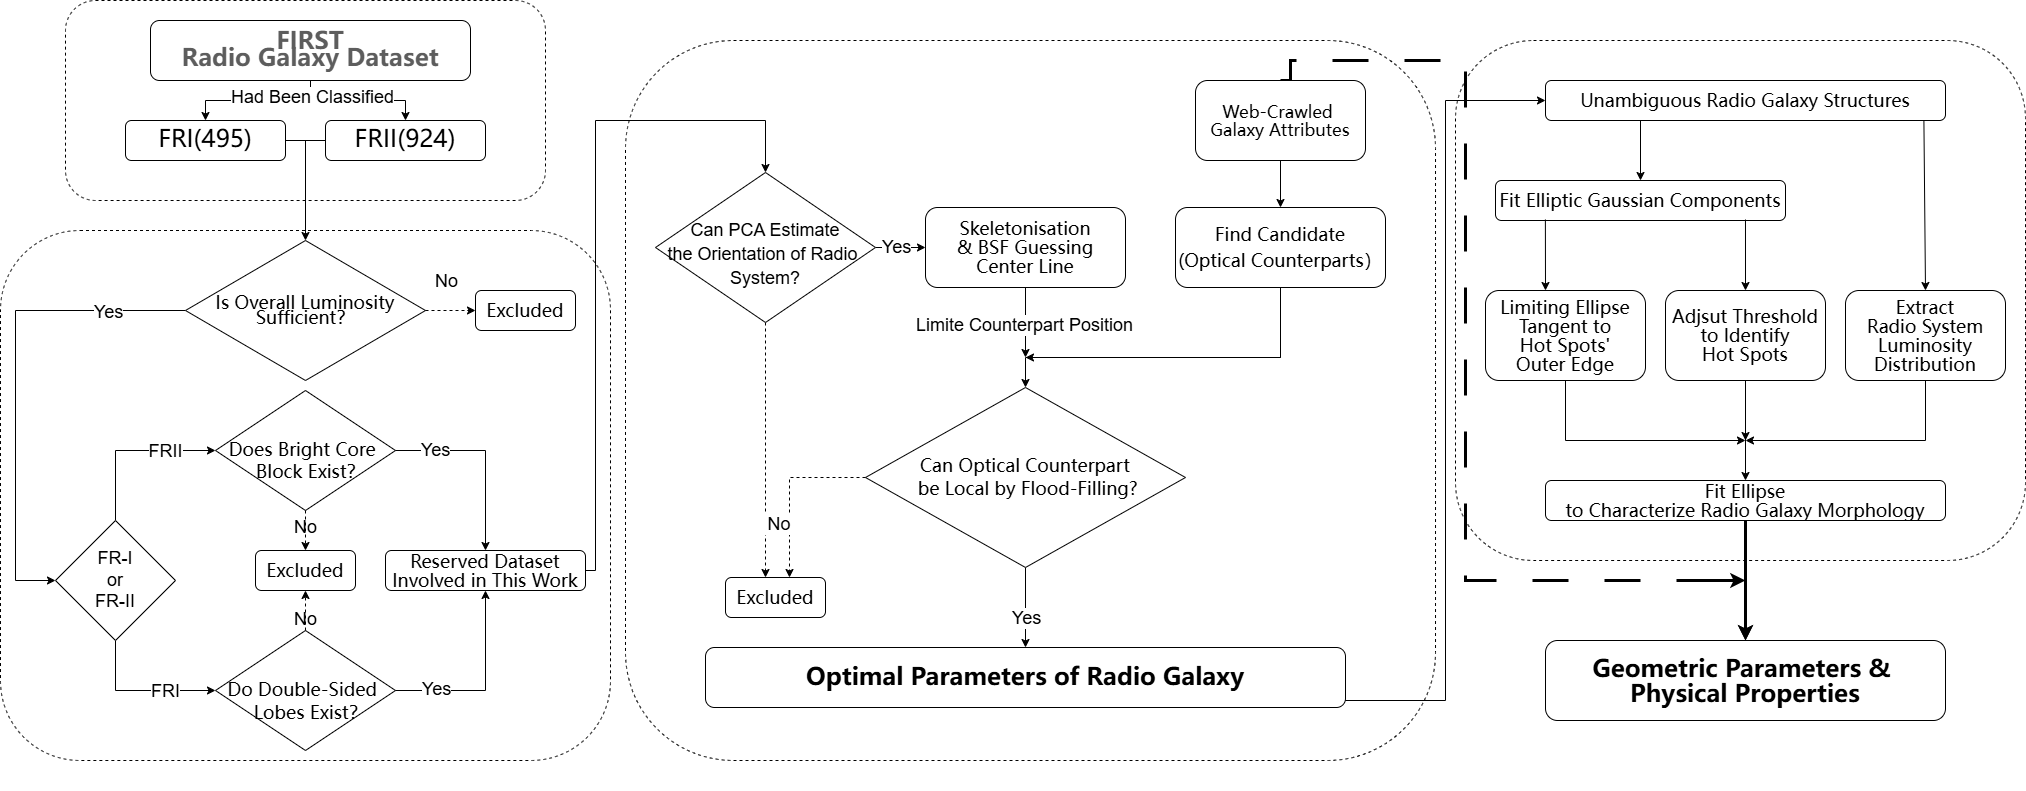
\includegraphics[width=0.9\linewidth]{Figure/Section 3/FR_type_operate.drawio.png}
    \caption{Flowchart for processing FR-classified RGs in \autoref{sec:Method}. The ultimate goal of this job is to conduct statistics on the relevant parameters of the RG.}
    \label{fig:Figure1}
\end{figure*}


\begin{figure}[!htbp]
    \centering
    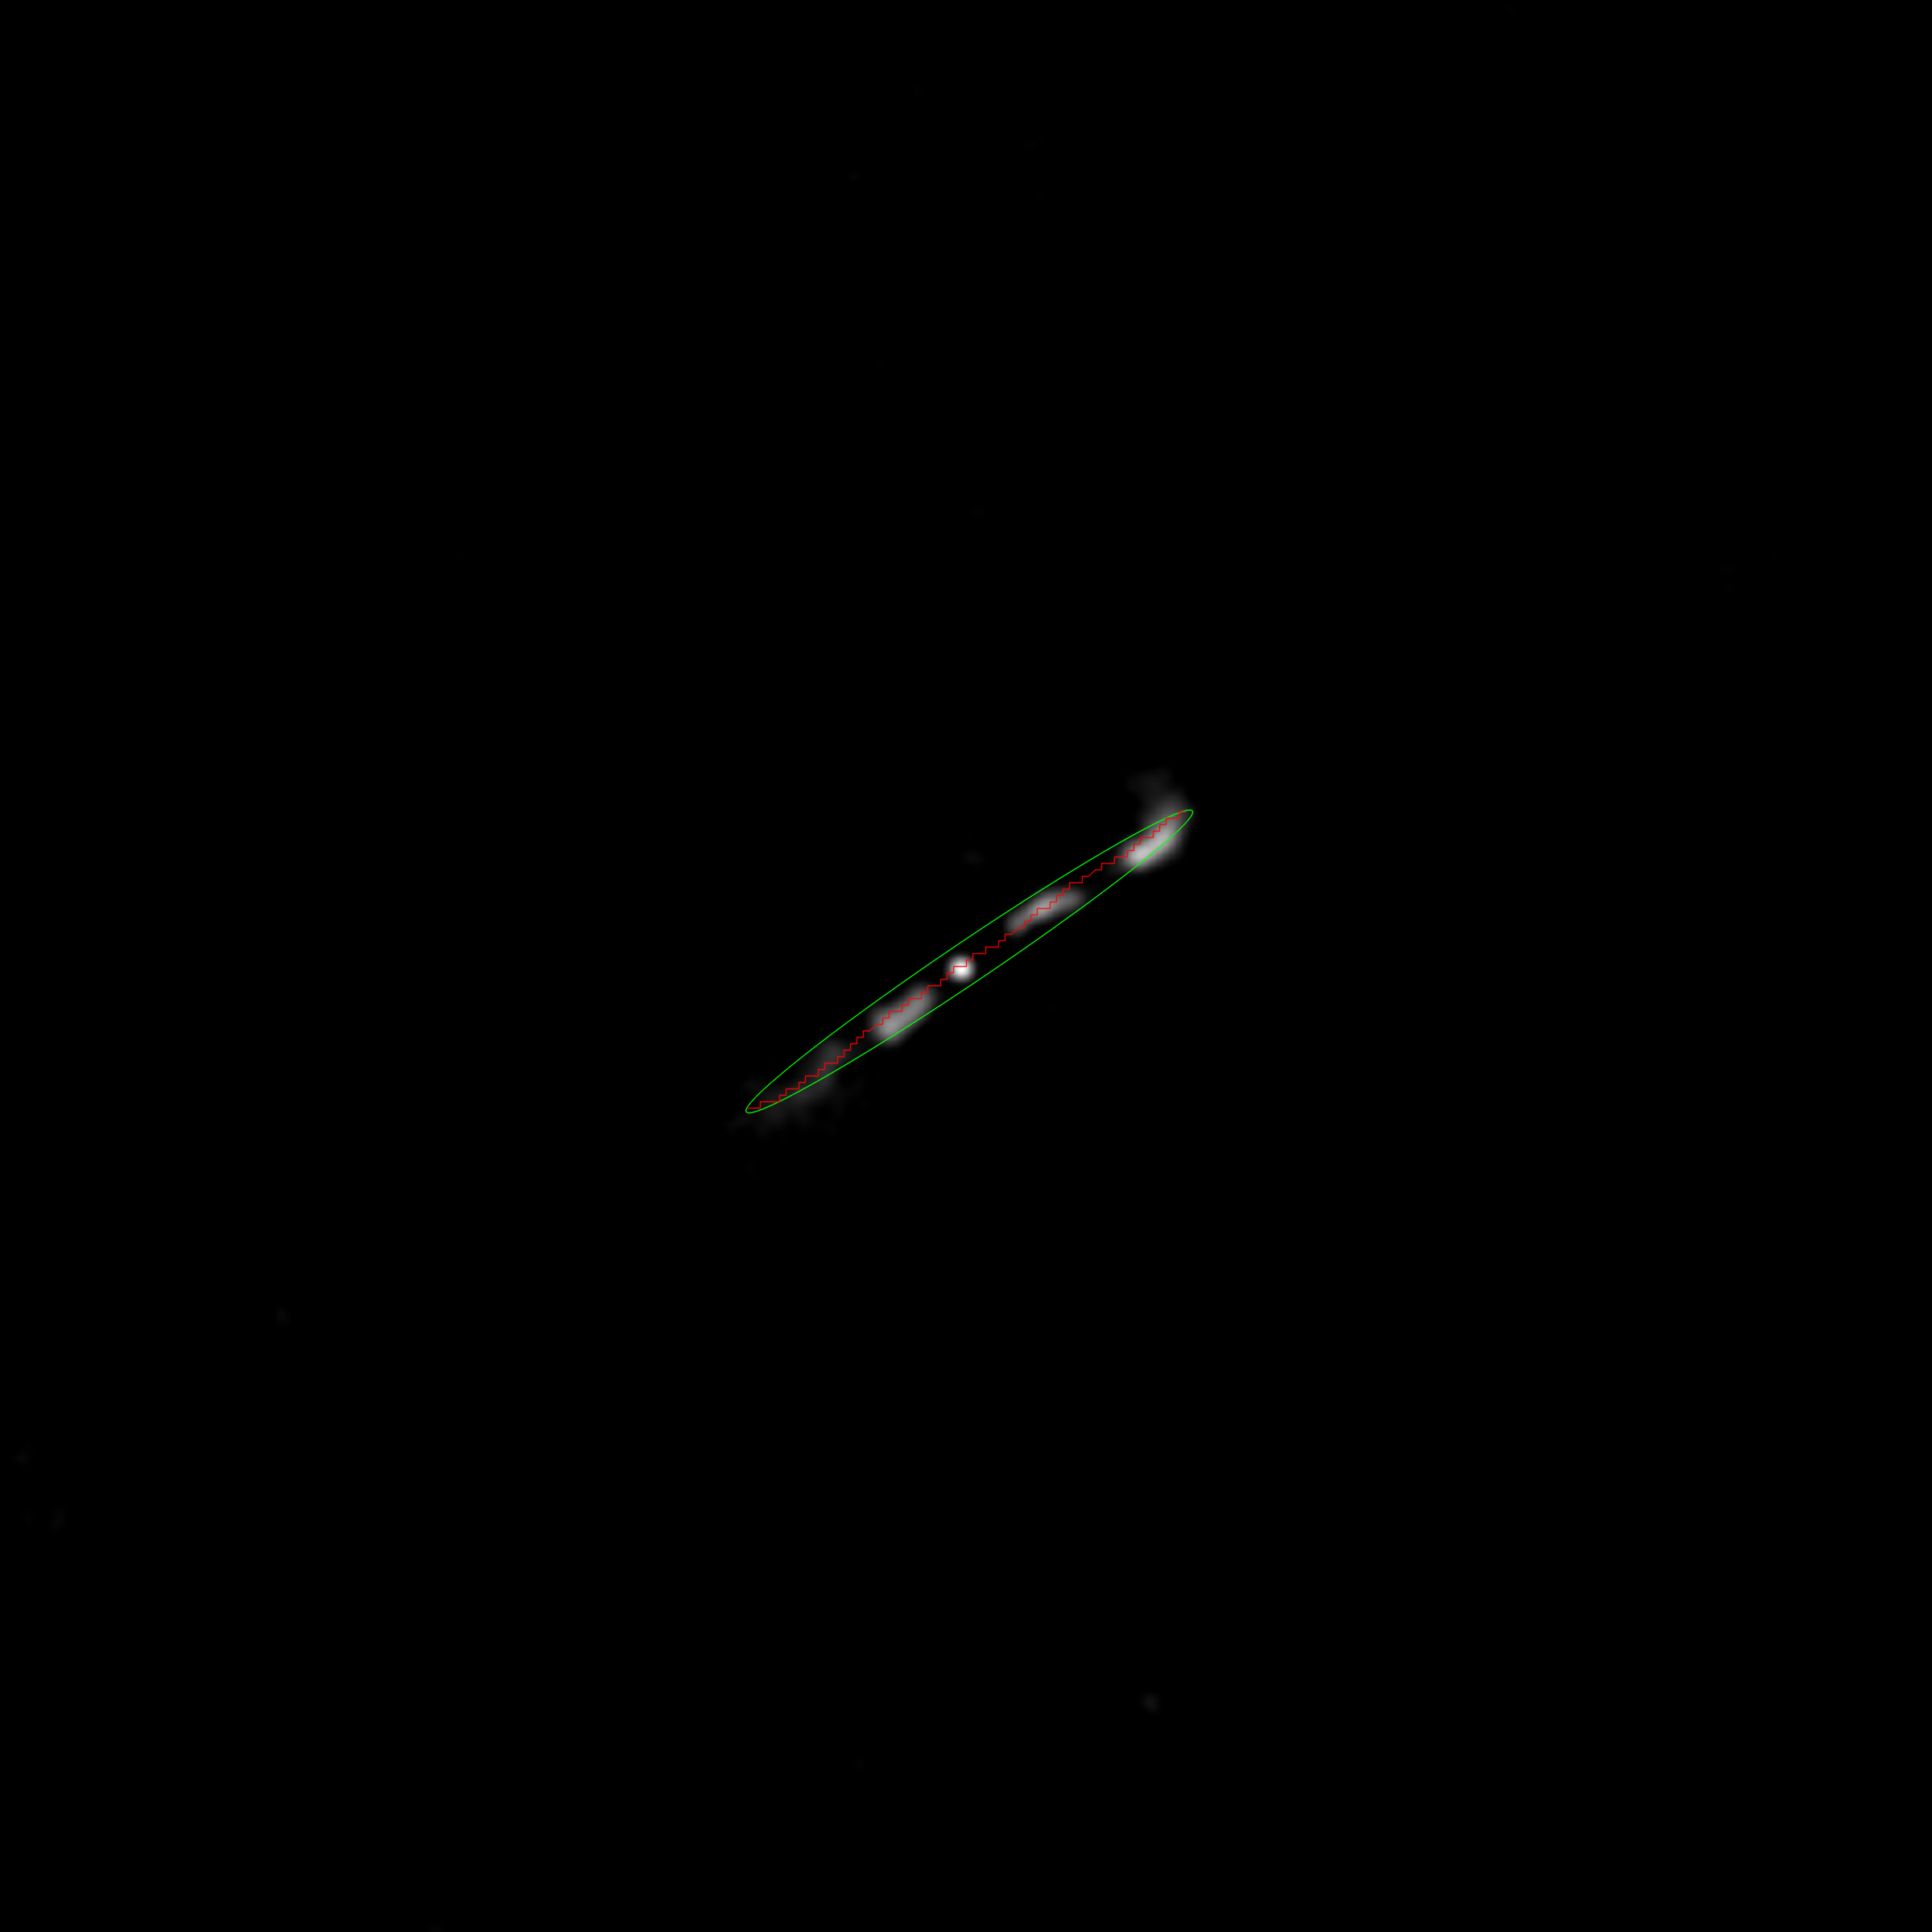
\includegraphics[clip, trim=100 100 100 100, scale=1.5, width=0.3\linewidth]{Figure/Section 3/149.318_19.114_0_MiraBest.png}
    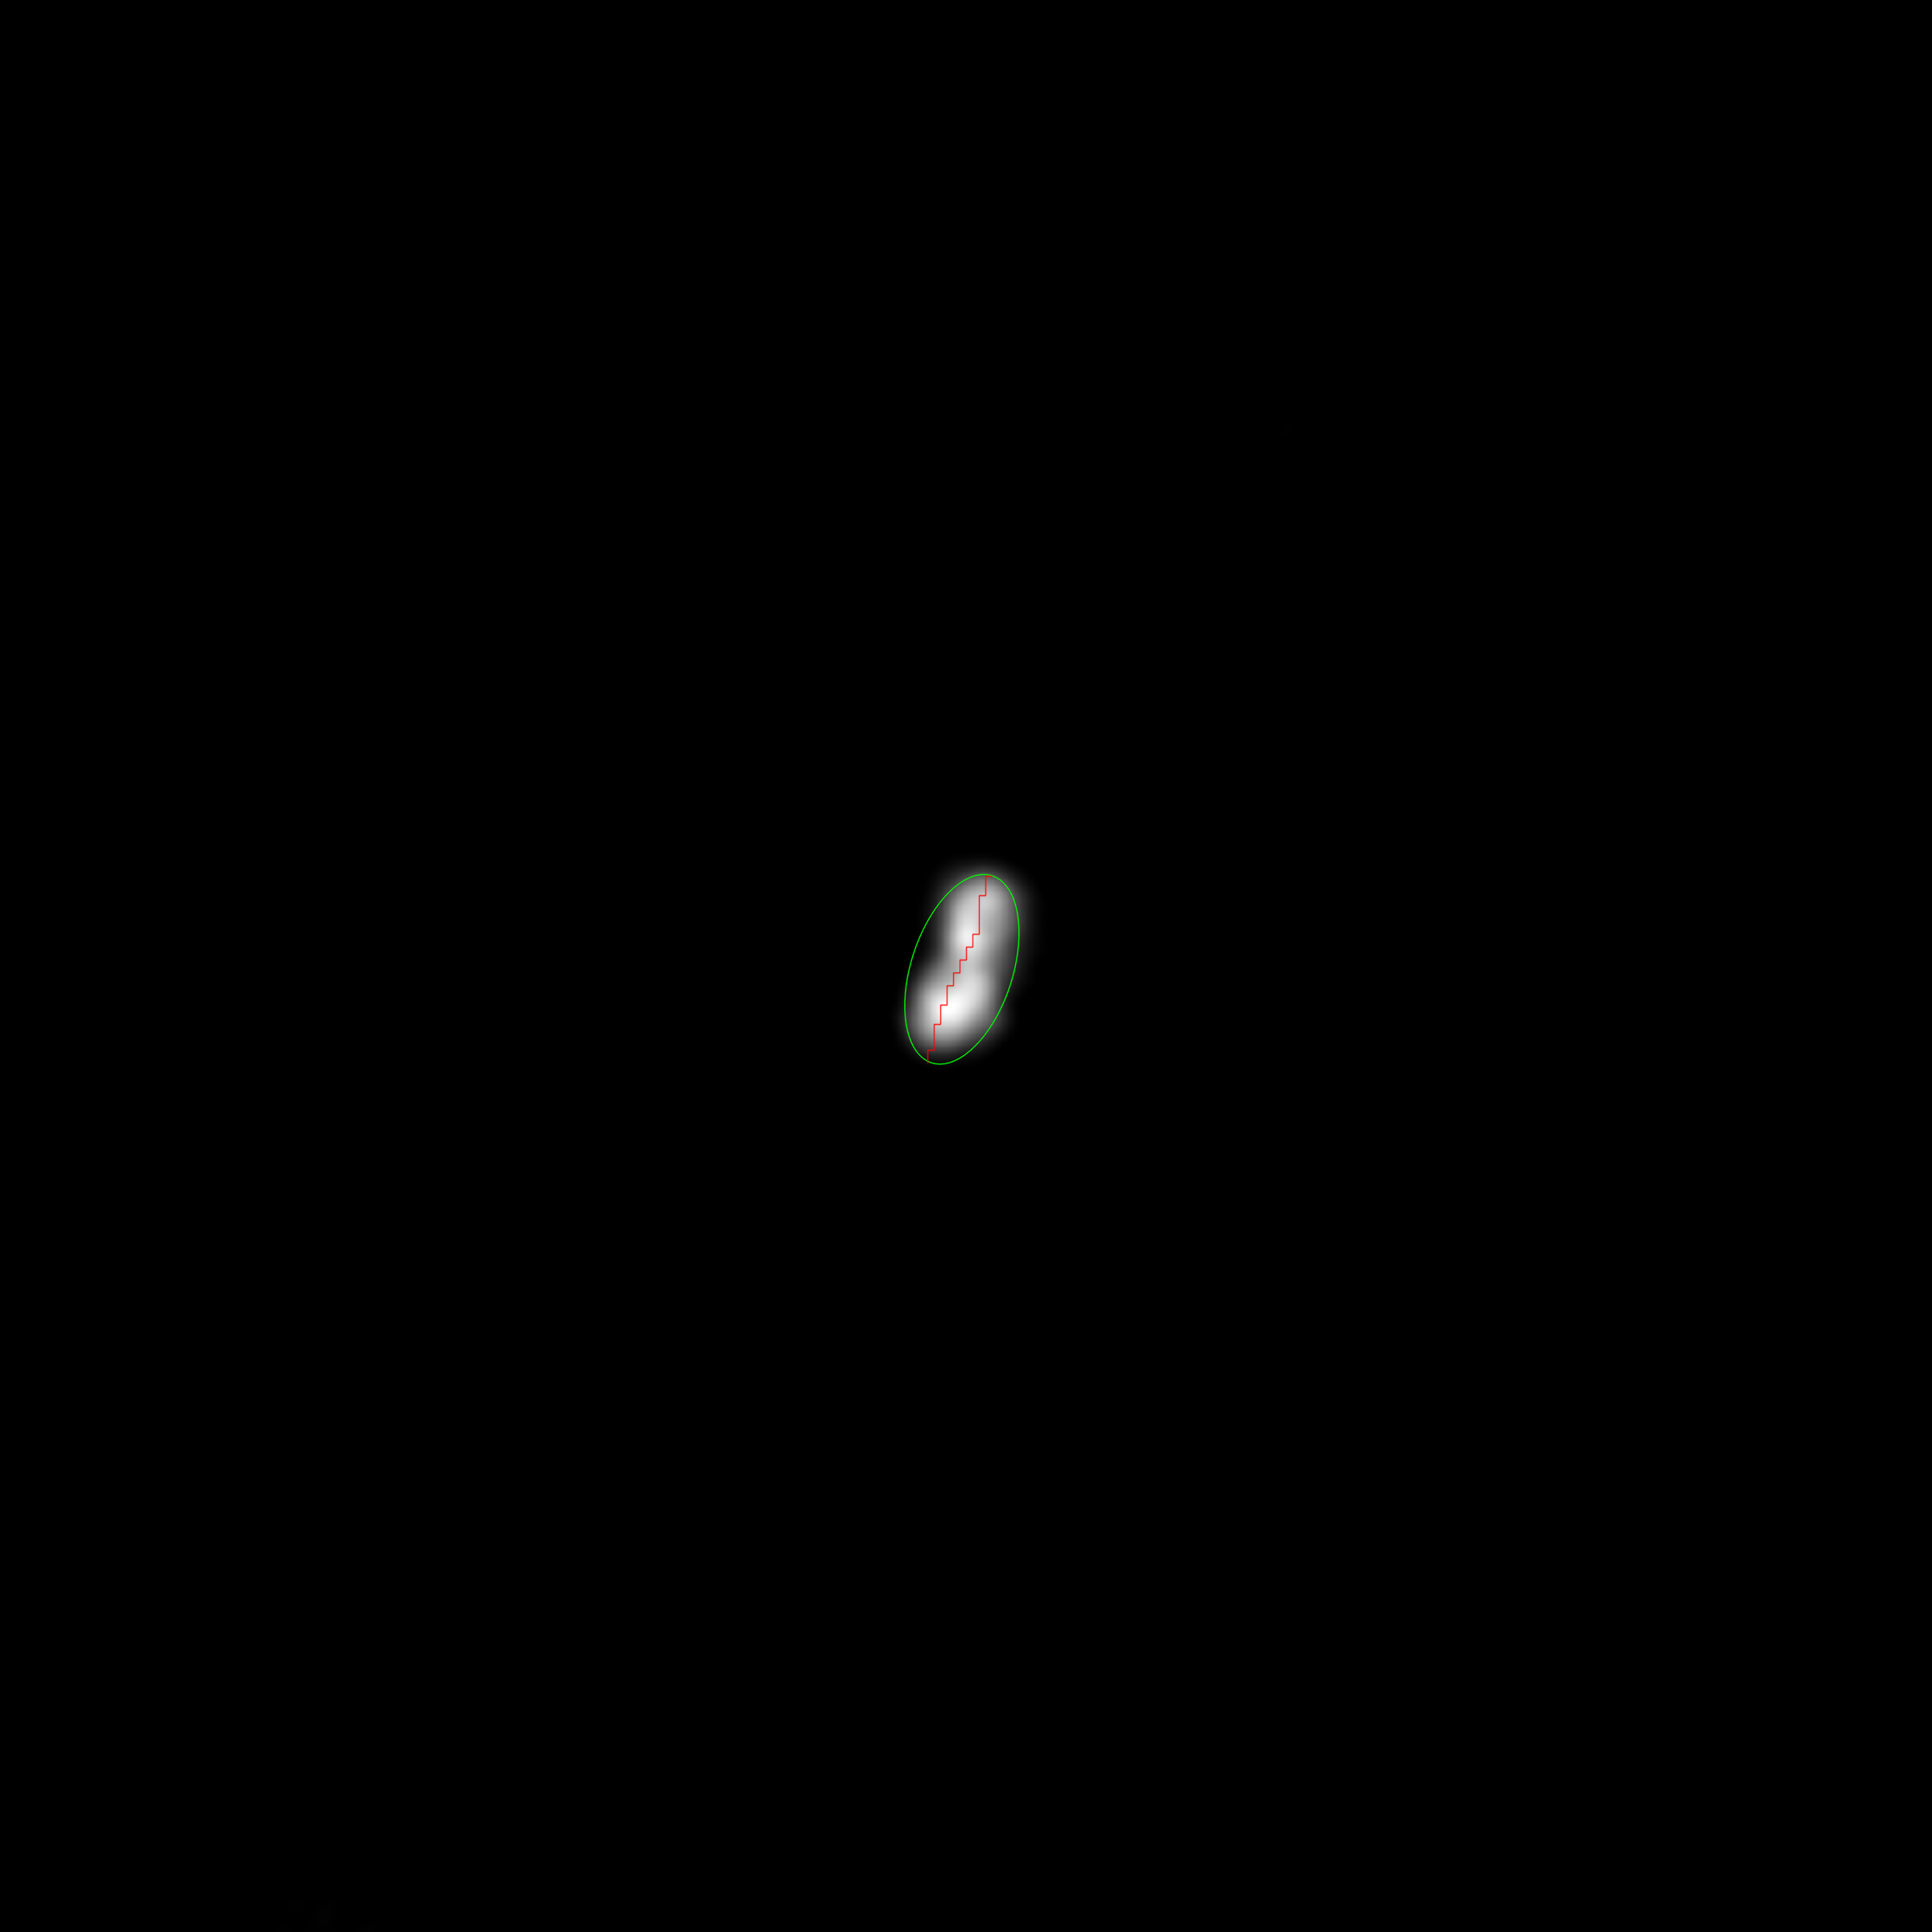
\includegraphics[clip, trim=125 125 125 125, scale=1.5, width=0.3\linewidth]{Figure/Section 3/150.738_19.865_0_Gendre.png}
    \includegraphics[clip, trim=135 135 135 135, scale=1.5, width=0.3\linewidth]{Figure/Section 3/175.545_55.458_0_Capetti2017a.png}
    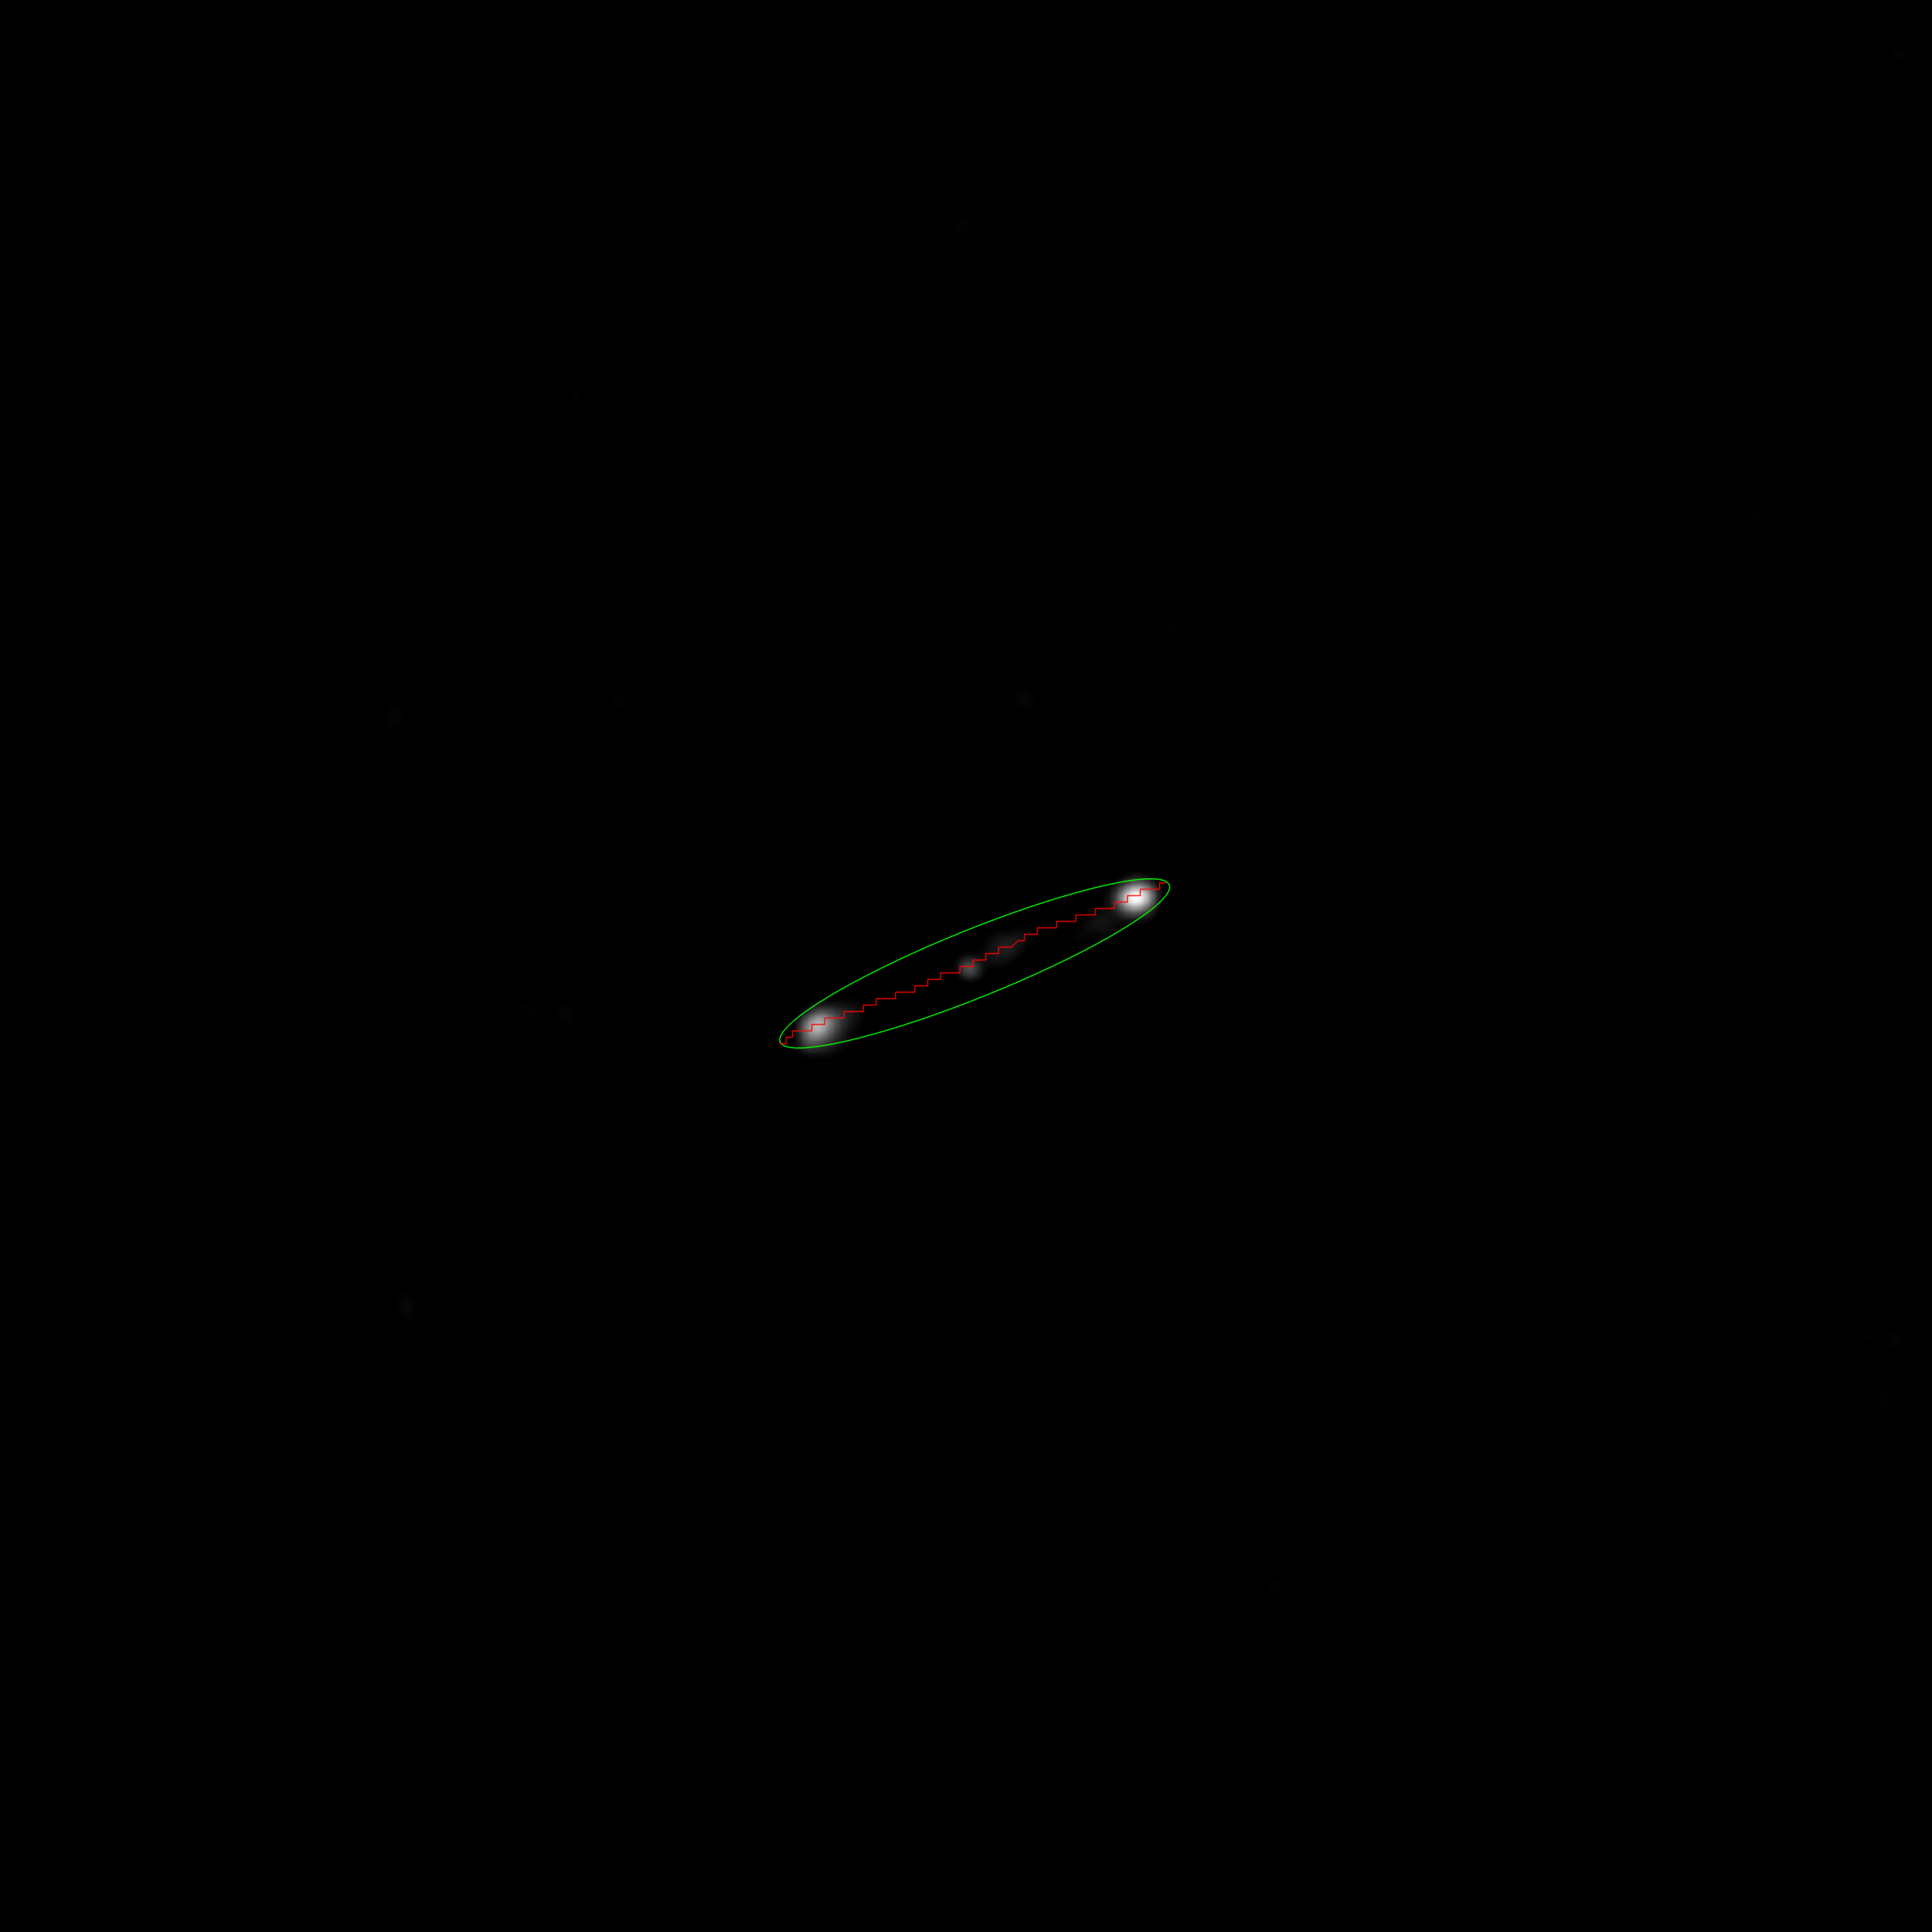
\includegraphics[clip, trim=115 115 115 115, scale=1.5, width=0.3\linewidth]{Figure/Section 3/180.424_22.946_1_MiraBest.png}
    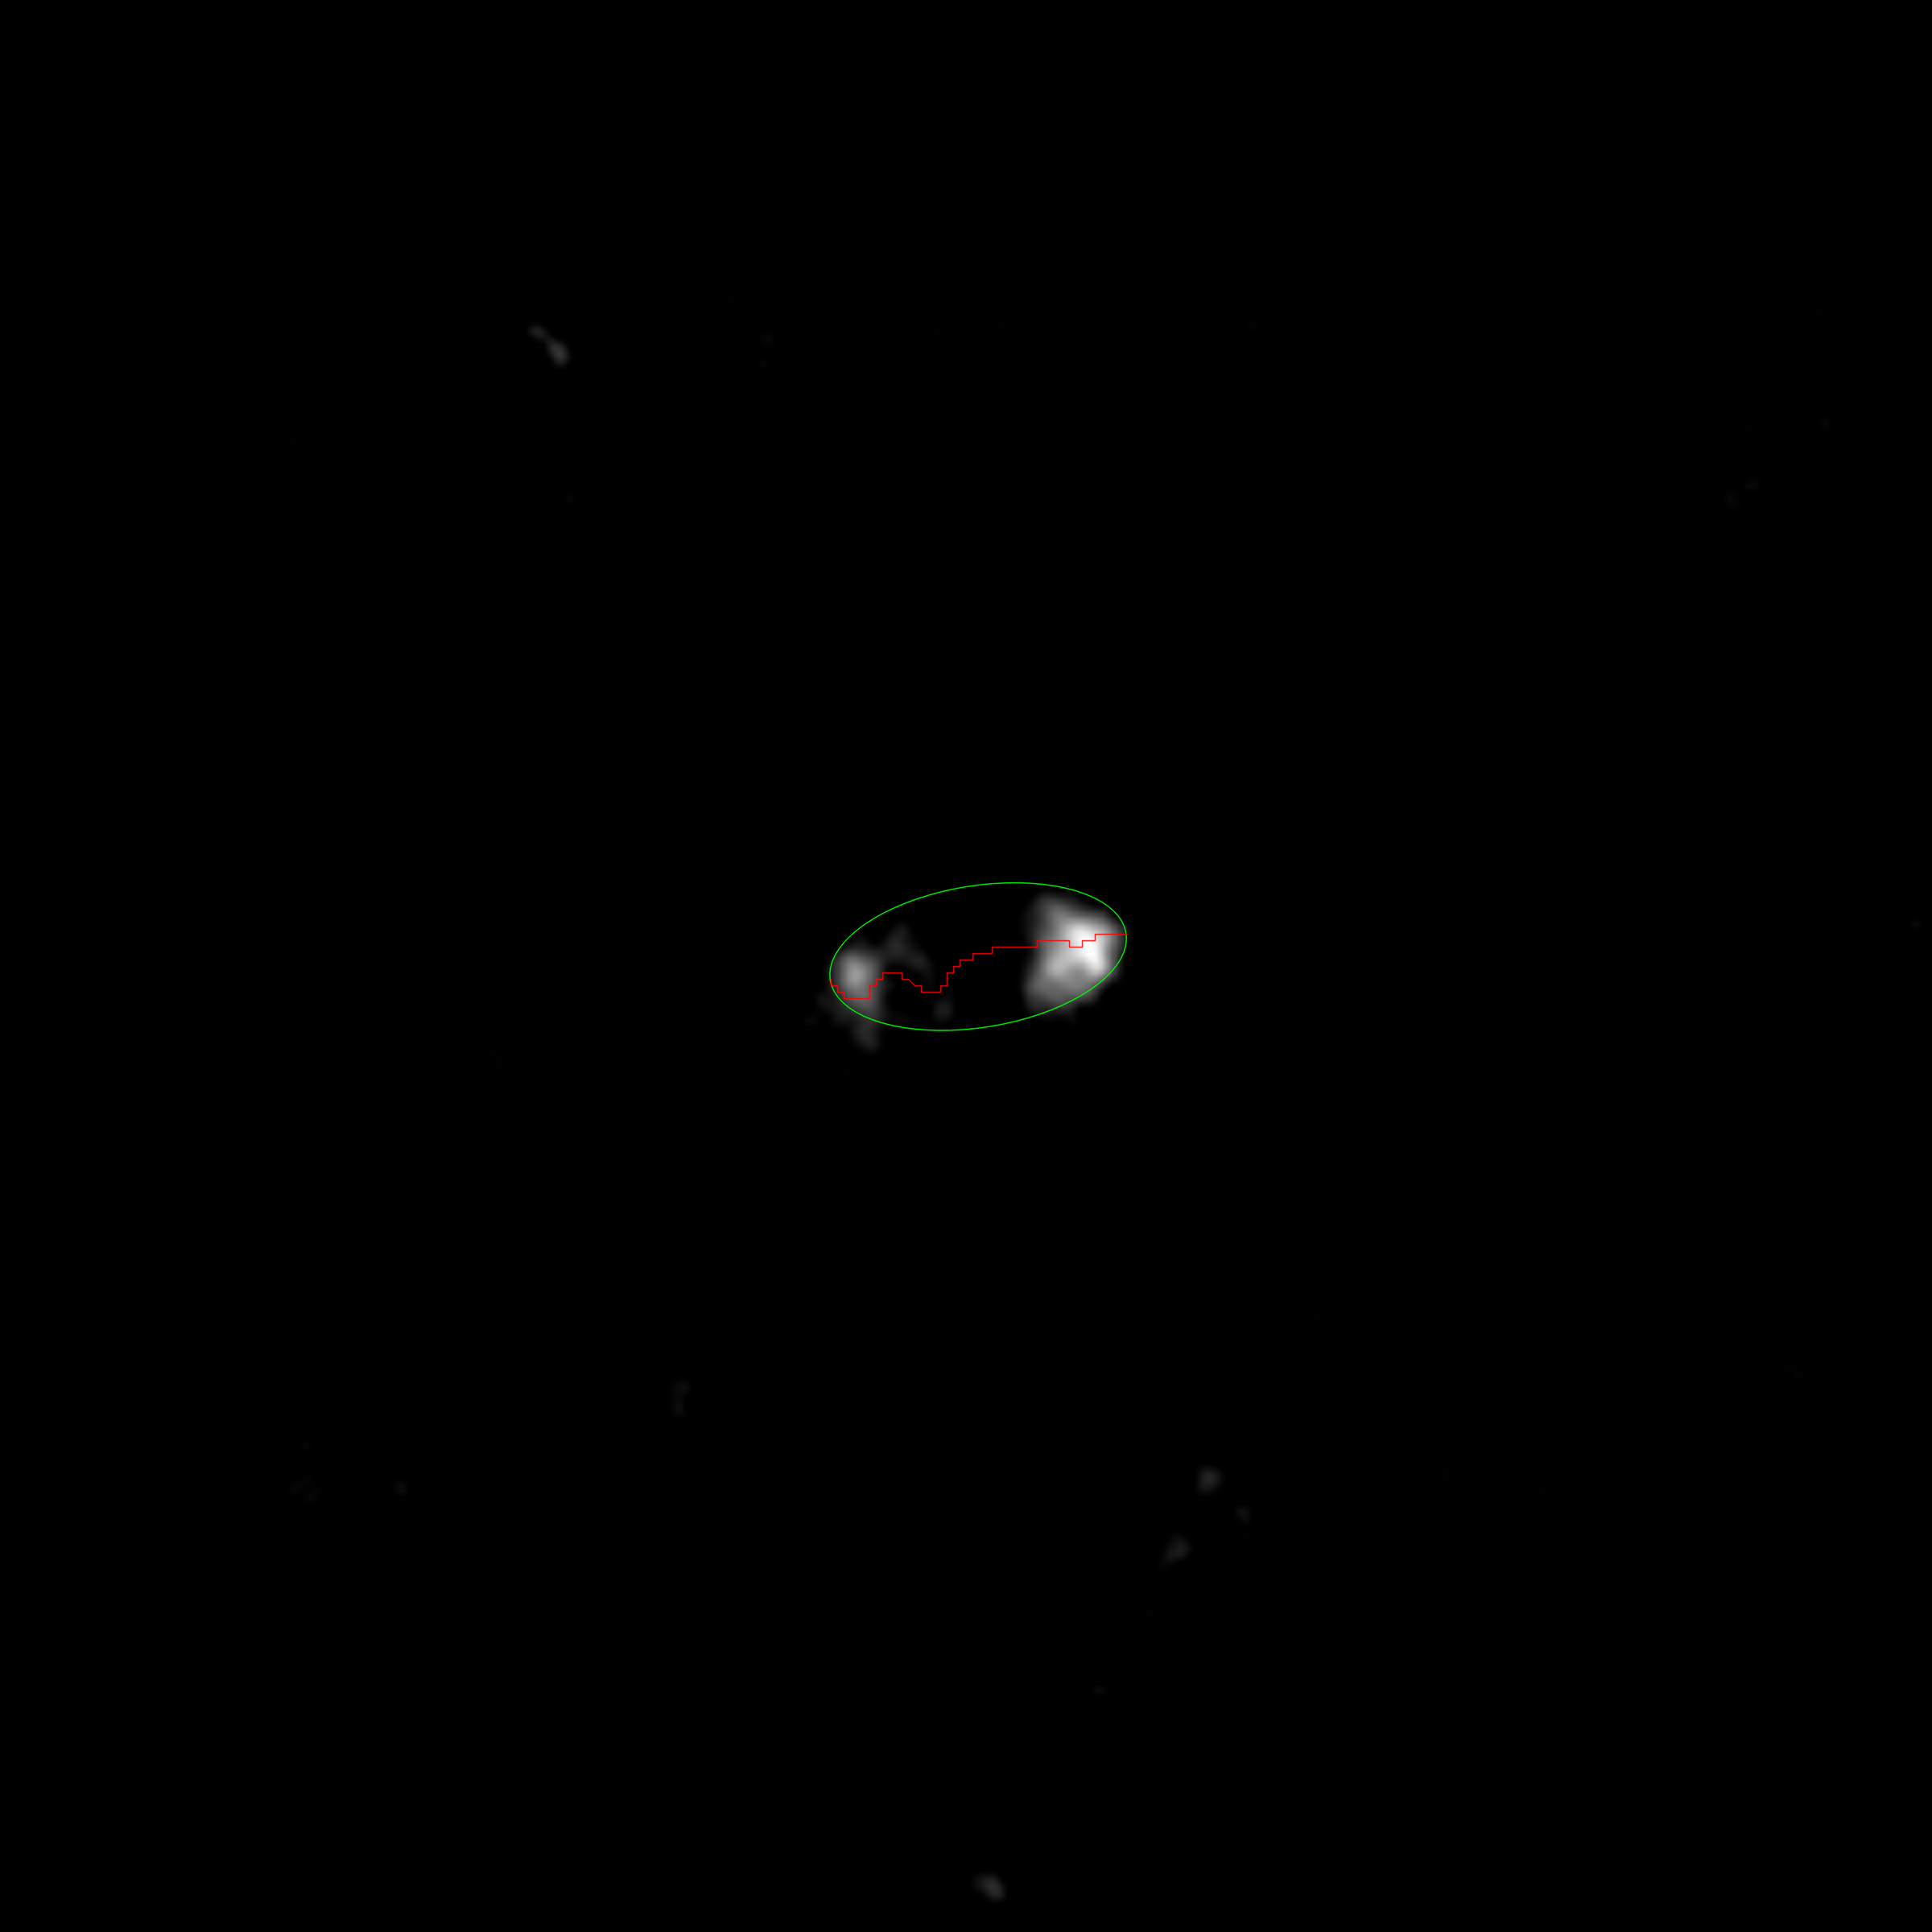
\includegraphics[clip, trim=120 120 120 120, scale=1.5, width=0.3\linewidth]{Figure/Section 3/213.728_22.633_1_MiraBest.png}
    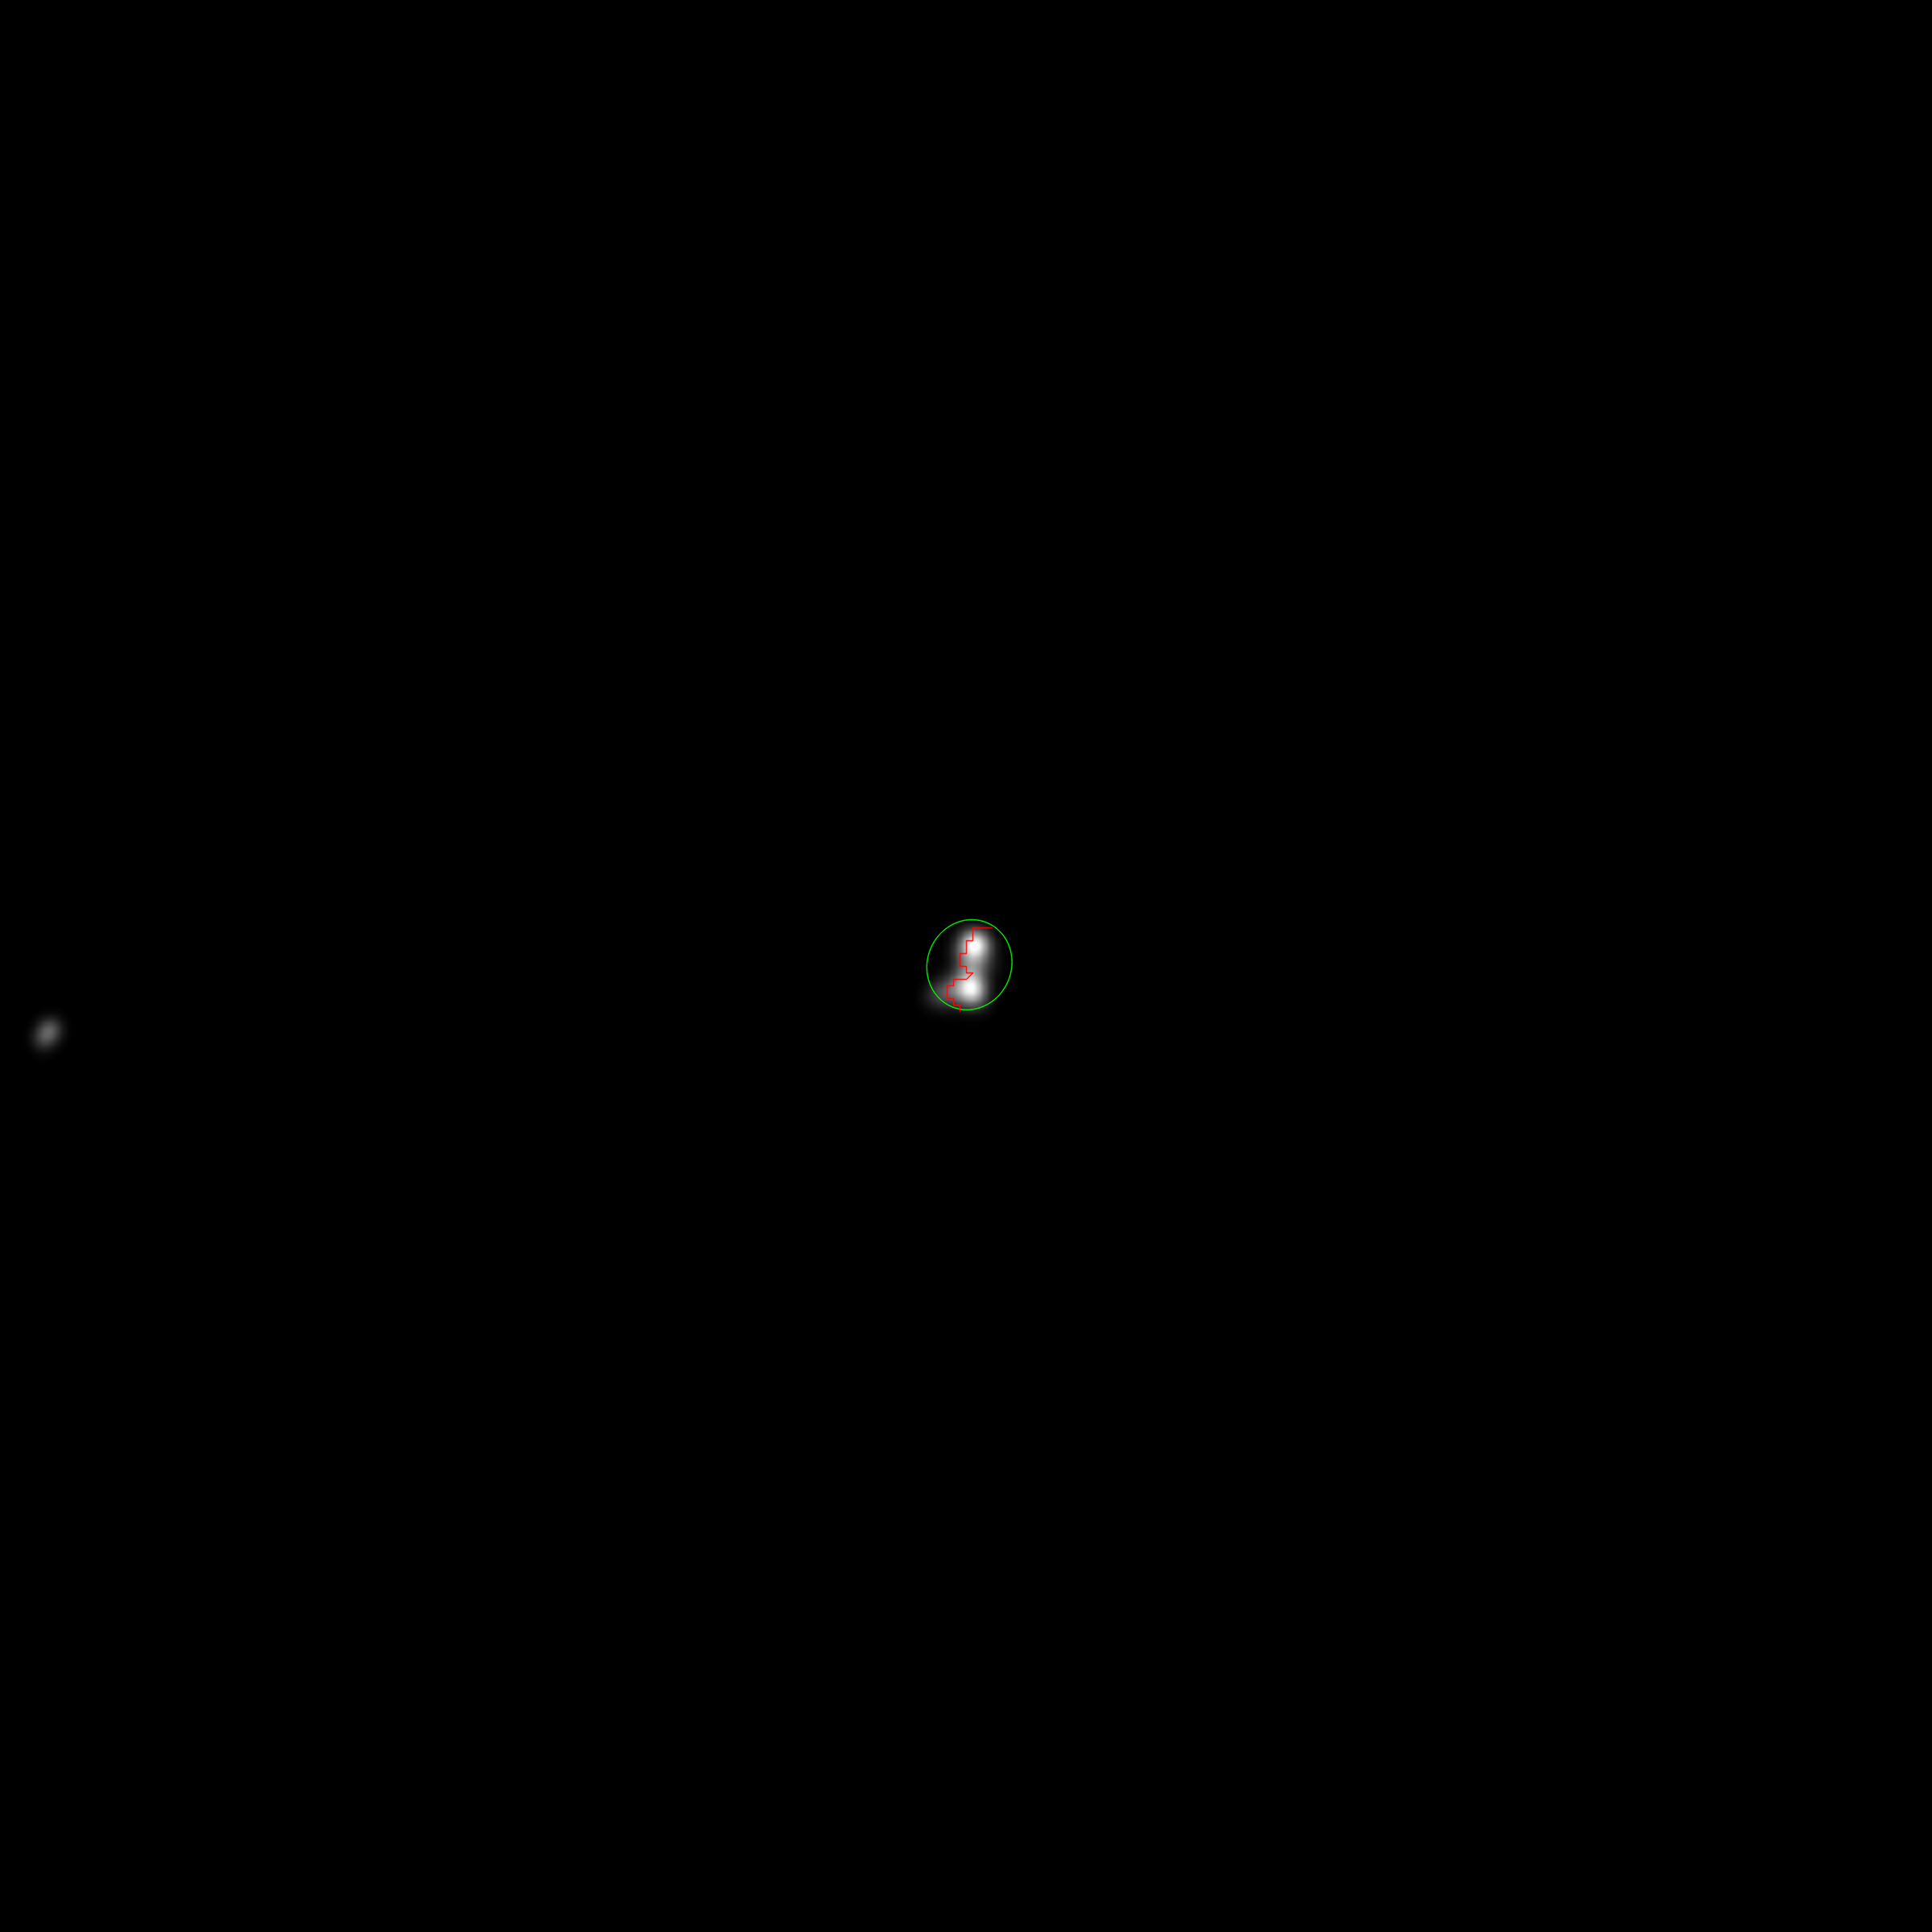
\includegraphics[clip, trim=135 135 135 135, scale=1.5, width=0.3\linewidth]{Figure/Section 3/125.391_47.043_1_Gendre.png}
    \caption{
    Top Panel: showing the FRI-type source.
    Bottom Panel: showing the FRII-type source.
    The green ellipse represents the algorithm-identified RG ellipse; the red/blue cross markers in the bottom panel denote the tangent point between the hot spot and ellipse\textemdash these points also serve as the major axes of the FRIIs' ellipses.
    }
    \label{fig:Figure2}
\end{figure}


\subsection{Searching Optical Counterparts}\label{sec:Section3_2}
To position the core of RGs, an effective approach leverages optical host galaxy positional data. For example, when searching for target galaxy-associated sources, \citep{kumar_growth_2022} used NED’s gravitational wave follow-up service to conduct quick-look searches for candidates. Similarly, NED is used here to find optical counterparts and retrieve their data. In \autoref{sec:Section3_1}, the sample’s filtered optical counterparts show redshift distributions (see \autoref{fig:Figure3}), with most redshifts < z=1. Optical counterpart mass and redshift data originate from catalogs archived in VizieR. This becomes challenging when multiple catalogs correspond to one optical counterpart, one catalog includes multiple estimation methods, or both; thus, the average mass is used for individual RGs. Naturally, data with both central black hole and stellar mass measurements is more representative\textemdash entries lacking either were excluded. In \autoref{fig:Figure4}, the central black hole mass and galaxy stellar mass data for FRIs and FRIIs in the sample exhibit a slight degree of misalignment. However, their distribution ranges are so similar that this stands in sharp contrast to the subsequently analyzed parameters with significant differences. This suggests that the mass information observed in the sample may not be the key factor affecting the radio activity of AGNs at 1.4 GHz.

\begin{figure*}[!htbp]
    \centering
    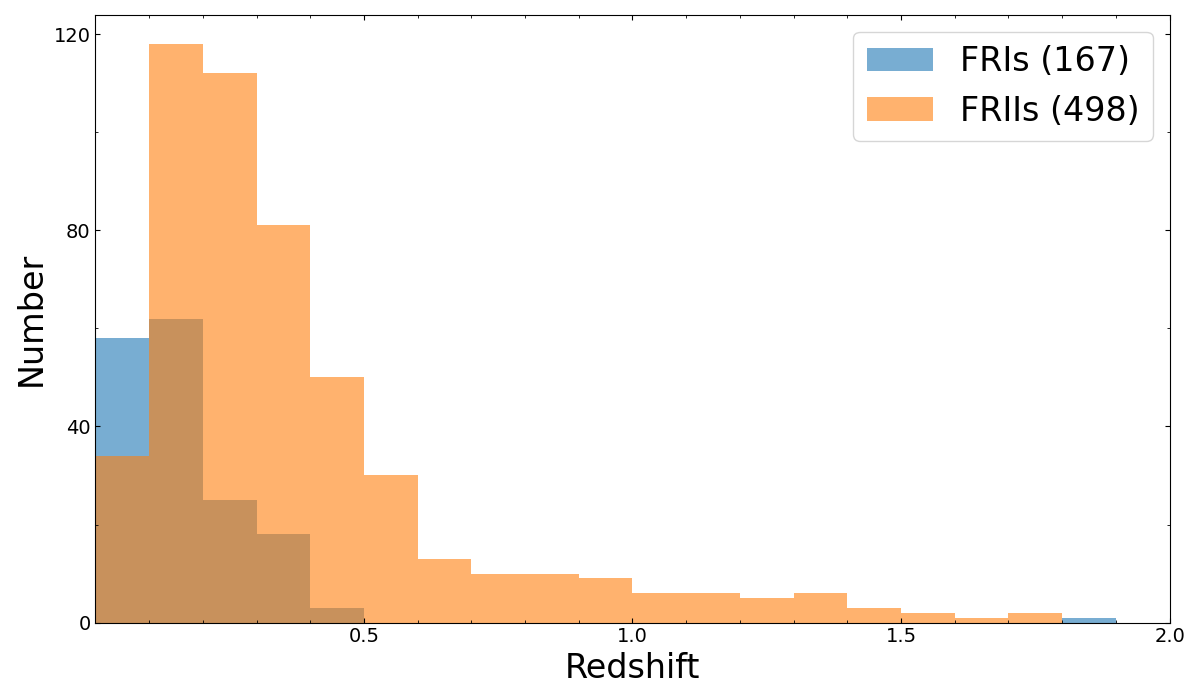
\includegraphics[width=0.9\linewidth]{Figure/Section 3/Redshift.png}
    \caption{Figure 1 presents the redshift distribution of RGs with identifiable optical counterparts selected from the visually screened dataset. The blue histogram corresponds to FRI-type sources, comprising 270 objects, while the red histogram denotes FRII-type sources, with a total of 564 objects.}
    \label{fig:Figure3}
\end{figure*}
\begin{figure*}[!htbp]
    \centering
    \begin{tabular}{cc}
        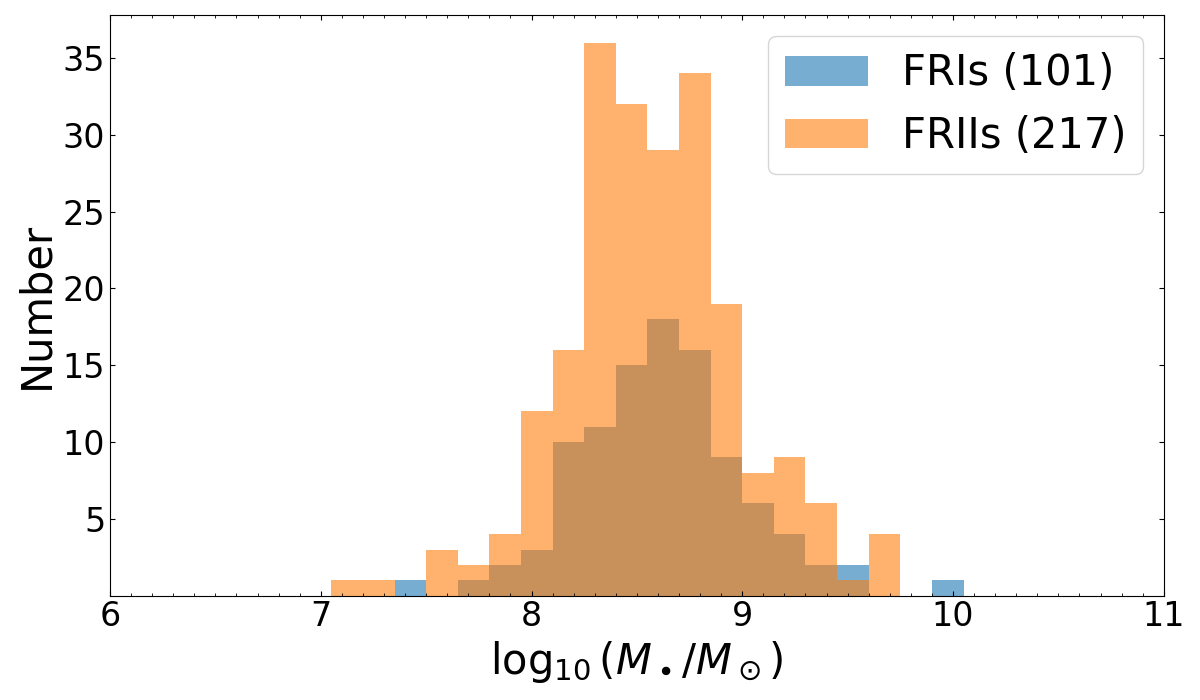
\includegraphics[width=0.45\linewidth]{Figure/Section 3/MassDistribution1.png}&
        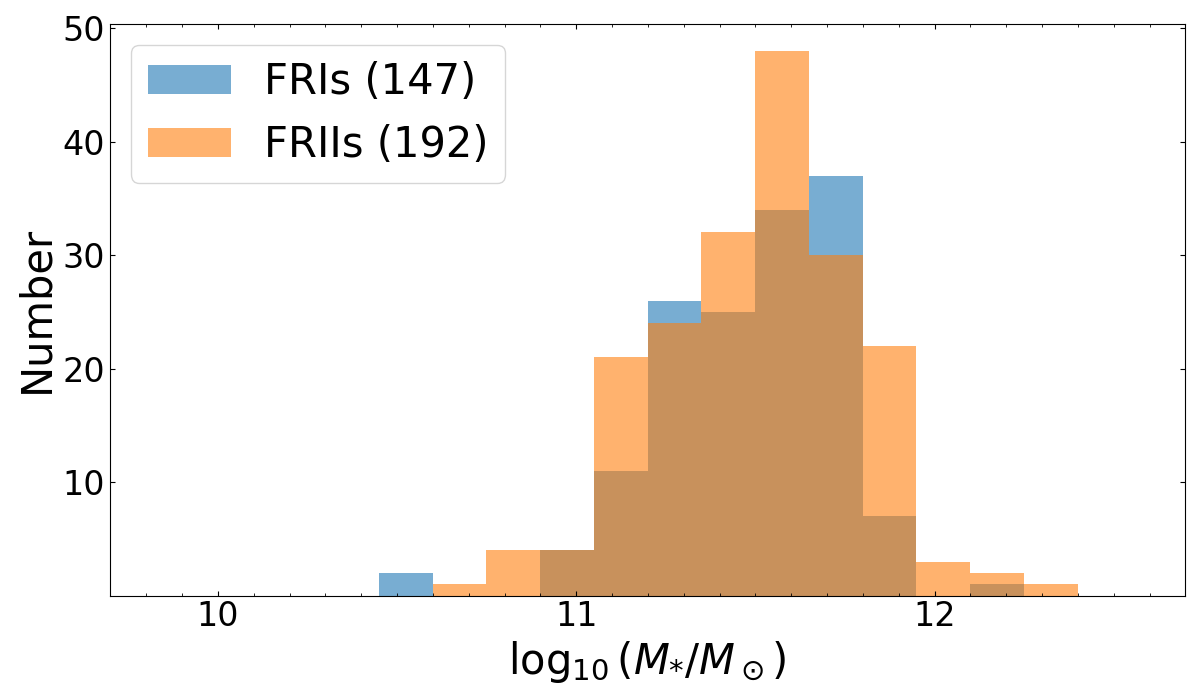
\includegraphics[width=0.45\linewidth]{Figure/Section 3/MassDistribution2.png}
        \end{tabular}
    \caption{The counts distribution plots for central black hole mass (left panel) and galaxy stellar mass (right panel), with the horizontal axis representing the logarithmic value of mass in solar units. In the figure, only the data with a one-to-one correspondence between central black hole mass and galaxy stellar mass are shown (Some optical counterparts may not be found any mass, or only one of them, and they were excluded). All data are the average values derived from the data of designated optical counterparts extracted from VizieR.}
    \label{fig:Figure4}
\end{figure*}


\subsection{Flood-filling Algorithm}\label{sec:Section3_3}
To extract the contours of RGs, employing the Flood-filling algorithm serves as an effective method for determining the extent of the associated RG \citep[e.g.,][]{mingo_revisiting_2019,hales_blobcat_2012}; Starting from known internal points, the Flood-filling algorithm only expands to adjacent non-boundary points, while boundary points are consistently excluded; this facilitates the identification of the contours of RGs under specific conditions \citep{lieberman_how_1978,fishkin_family_1984}. In this procedure, it is specified that the Flood-filling algorithm will disperse seed points in all connected regions of the image with non-zero brightness, while the brightness threshold is set to 5\% of the brightness value of the brightest point in the image.


\subsection{Principal Component Analysis}\label{sec:Section3_4}
Most applications of PCA in astronomy relate to identifying eigenvectors across a population of objects \citep[e.g., PCA tomography][]{steiner_pca_2009}, PCA will be employed to detect the principal direction that best align with RG structures in the context of the present work. PCA is a powerful technique for extracting structure from potentially high-dimensional datasets, and a small number of principal components is often sufficient to account for most of the structural information in the data \citep{hofmann_kernel_2008}. Specifically, for the morphological analysis of RGs\textemdash whose observational data typically encompasses multidimensional information (e.g., spatial coordinates and brightness gradients)\textemdash PCA integrates these discrete data points into a low-dimensional principal component space. It prioritizes and preserves the information driven by the highest variance while filtering out noise and redundant signals unrelated to morphology. In this paper, in addition to the targeted RGs, other radio sources (e.g., compact sources) present in the acquired FIRST images interfere with the processing of the target. Compared with RGs, these interfering sources exhibit simpler structures and significantly smaller scales. Consequently, when PCA is employed to process the brightness distribution, the variance corresponding to the identified largest distribution direction is substantially greater than that of the second largest variance. PCA enables the direct retrieval of the core morphological features of RGs without relying on complex auxiliary data, which aligns with the previously outlined requirement for efficient and concise morphological extraction.


\subsection{Central Line}\label{sec:Section3_5}
Skeletonization is a well-established method for image structure characterization, and Breadth-First Search (BFS) enables the identification of the central line of RG skeleton\textemdash this line, in turn, facilitates the simplification of the features of the RG's brightness distribution. Skeletonization enables efficient compression of RG structure while preserving its core structural information. Specifically, using iterative skeletonization methods, foreground regions can be reduced to single-pixel-wide skeletons while maintaining topological features; for analogous work, see \cite{vardoulaki_fr-type_2021}. Then, BFS algorithm enables the identification of a line within the skeletonization process that characterizes the center of RG brightness distribution. This constitutes a pruning process, as extraneous branches in the skeleton are irrelevant for characterizing the overall orientation of lobe structures. Thus, BSF algorithm can retain the primary backbone\textemdash most representative of lobe structure\textemdash hereafter referred to as the central line. Merely applying BFS algorithm alone is insufficient; it is additionally required to incorporate into the algorithm the constraint that the direction of the central line is roughly aligned with the PCA-derived principal direction, as well as the requirement that the central line passes through hot spots or other compact clumps.

\cite{barkus_application_2021} implemented similar techniques, though their ridge lines\textemdash designed primarily for identifying and morphologically classifying extended RGs in radio astronomy\textemdash are less suitable for RG systems with large gaps or curved head-tail structures.


\begin{figure*}[!htbp]
    \centering
    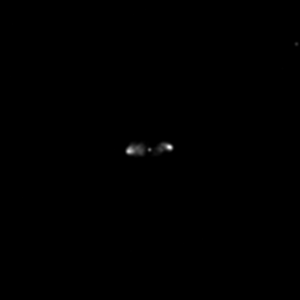
\includegraphics[clip, trim=100 100 100 100, scale=1, width=0.25\linewidth]{Figure/Section 3/178.47_38.197_1_MiraBest.png}
    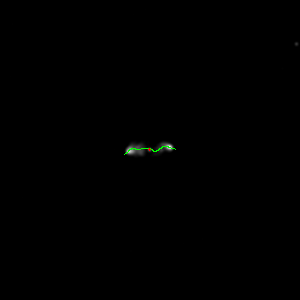
\includegraphics[clip, trim=100 100 100 100, scale=1, width=0.25\linewidth]{Figure/Section 3/CenterLine_178.47_38.197_1_MiraBest.png}
    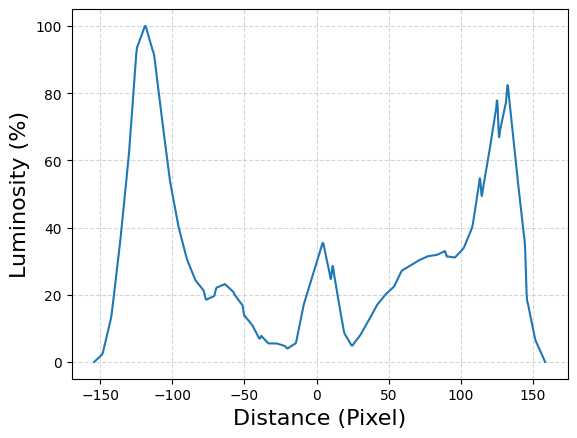
\includegraphics[width=0.33\linewidth]{Figure/Section 3/CenterLineLuminosity_178.47_38.197_1_MiraBest.png}
    \caption{Left: The cleaned RG (R.A. 178.47°, Dec. 38.197°);  Middle: The central line (Green) of RG;  Right: The luminosity distribution of central line.}
    \label{fig:Figure5}
\end{figure*}


\subsection{Elliptic Gaussian Model}\label{sec:Section3_6}
% 在这一方面的方法中，椭圆很重要
Elliptical structures are of considerable significance in morphological discussions. \cite{lin_new_2024} recalibrated the luminosity function for various types of RGs at 150 MHz by elliptical structure, and the power spectra of his model are closely aligned with those from the SKADS model. Some double-lobes of RGs' structure can exhibit a morphologically oriented and elongated elliptical structure (such as Cygnus A \citep{carilli_cygnus_1996}). \cite{begelman_overpressured_1989} once utilized the structure of cocoons of shocked gas to describe the RG Cygnus A; within their model, the bow shock surrounding hot spots is naturally described as an elliptical structure. Throughout previous analyses of RG structures, the recurrent emergence of a simple elliptical structure can be evidently observed. Clearly, an elliptical structure can be used to provide a general description of radio-loud sources.

To implement independent modeling of the core region and lobes of RGs, \cite{lin_populations_2010} suggested the angular separation between the highest surface brightness spots on either side of the galaxy as S, and the total linear size of the RG as T, defining $r_s \equiv S/T$ as the primary measure of RG morphology. A critical aspect of this work involves using Gaussian modeling to fit source components; unfortunately, many sources in the dataset employed in this study lack corresponding beam parameters that match those in the FIRST Catalog. 

To ensure the universality of the simulations, their methodology has been simplified: For FRII sources, hot spots are identified by locating the brightest points and outermost elliptical Gaussian components on either side of the optical counterparts of RGs; meanwhile, the maximum distance between the farthest pixels of a RG is adopted as the T value, which characterizes the overall size of the system. For FRI sources, S is defined as the major axis size of the largest elliptical Gaussian component at the system center. For optimal coverage of the entire RG, different strategies are employed based on FR type: For FRI, given its prominent bright core and typical Lobe-Core-Lobe structure, a three-component elliptical Gaussian model is used to fit the central clump and resolve it into one core and two lobes\textemdash with the component assigned the highest brightness weight designated as the core, and the other two as lobes. With the elliptical edges of the two lobes serving as tangent points, a minimal enclosing ellipse is determined. For FRII, an ellipse representing the RG is established using the elliptical Gaussian models of the hot spots: with the principal component direction fixed as the orientation and the elliptical boundaries of the hot spots serving as tangent points, a minimal enclosing ellipse is determined.

The process described above is illustrated in \autoref{fig:Figure6}. Meanwhile, \autoref{fig:Figure2} specifically presents the resultant elliptical structure resulting from the processing steps as illustrated in \autoref{fig:Figure1}.
The coordinates of these RGs are as follows: (R.A. 149.318°, Dec. 19.114°); (R.A. 150.738°, Dec. 19.865°); (R.A. 175.545°, Dec. 55.458°); (R.A. 180.424°, Dec. 22.946°); (R.A. 213.728°, Dec. 22.633°); (R.A. 125.391°, Dec. 47.043°).


\begin{figure}[!htbp]
    \centering
    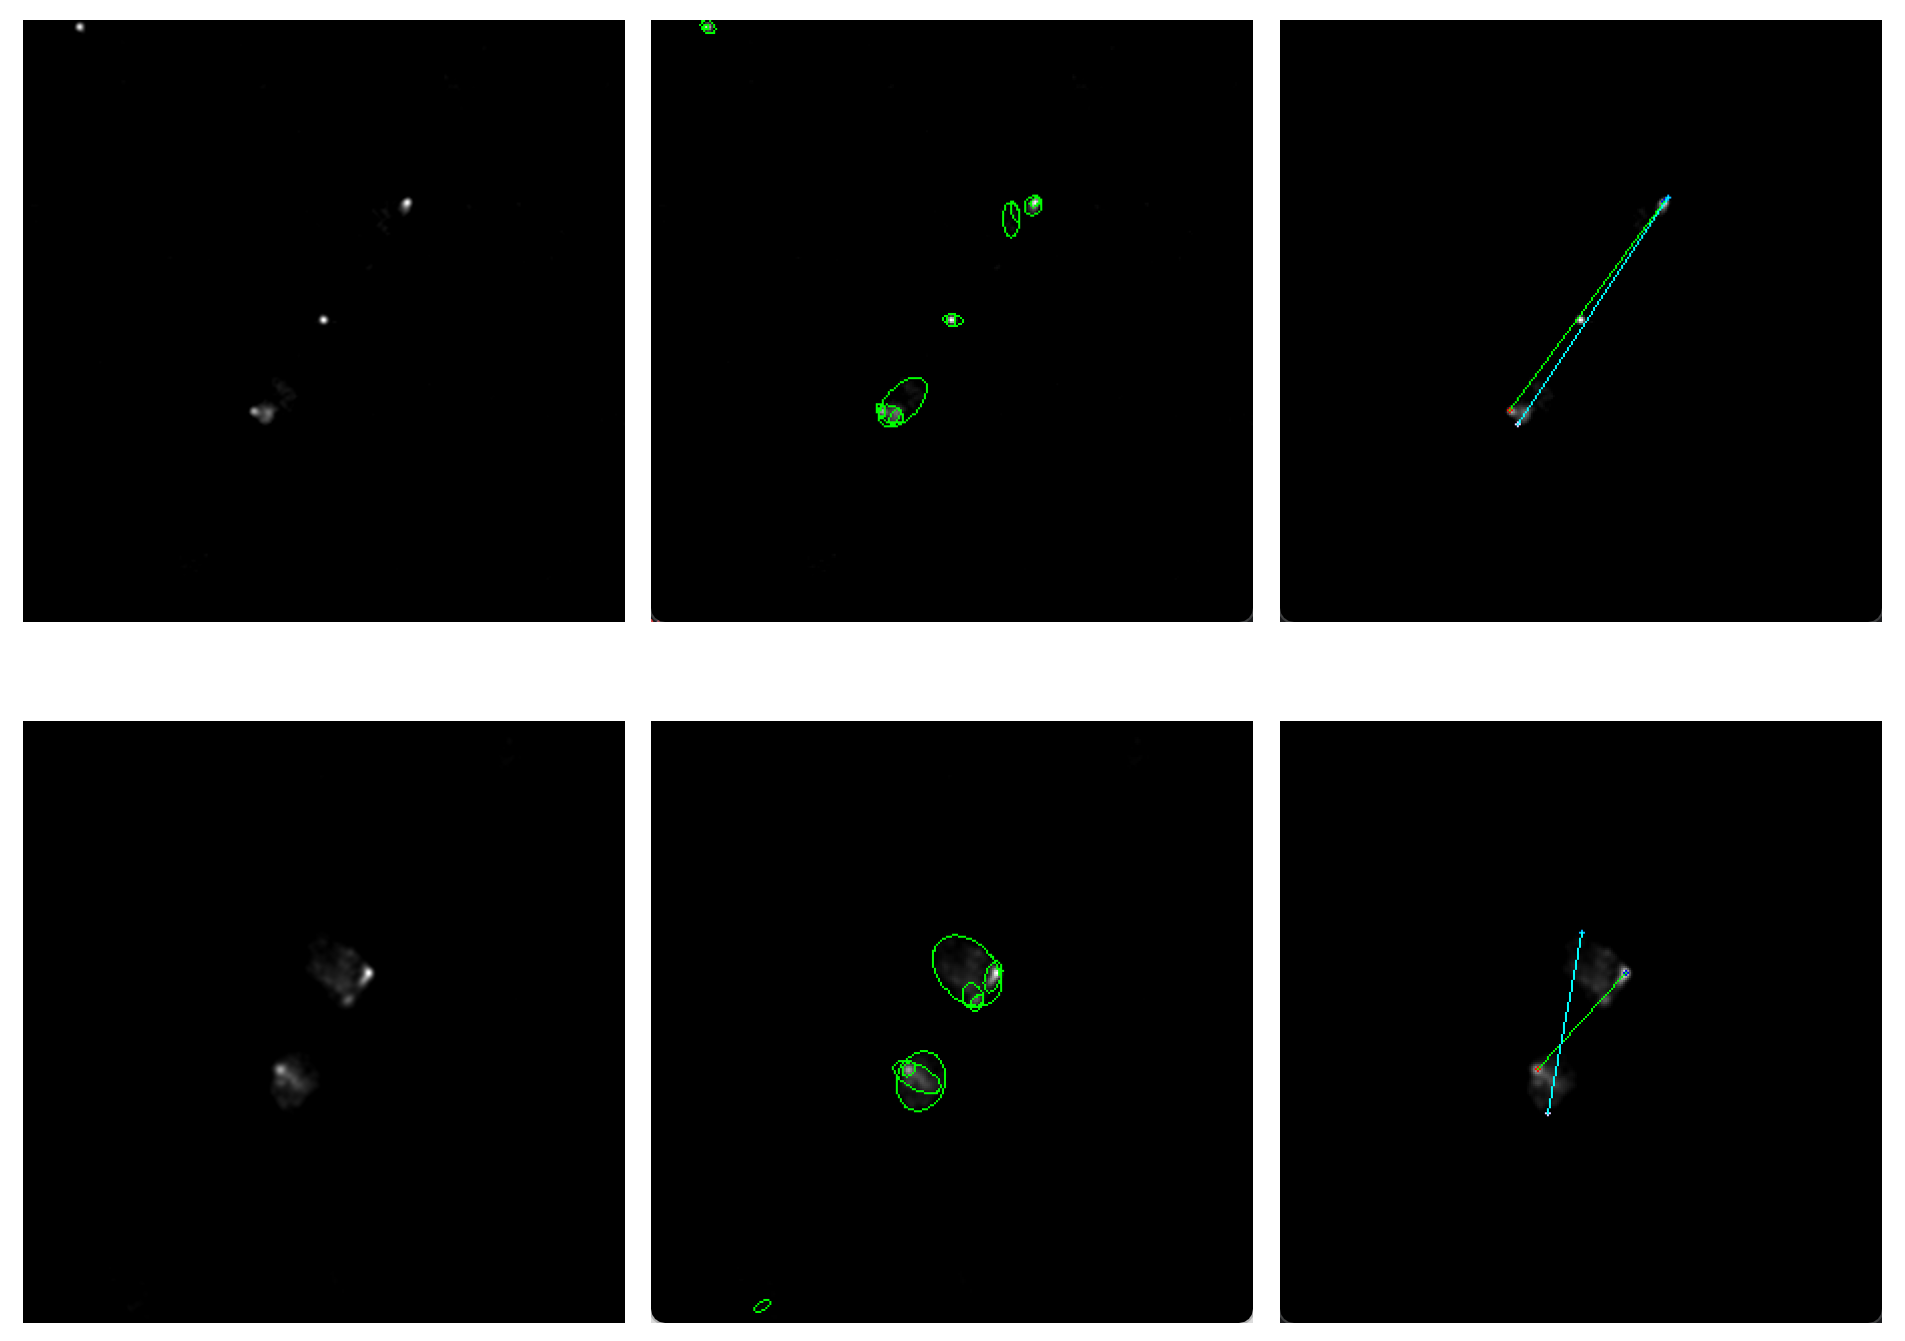
\includegraphics[width=0.9\linewidth]{Figure/Section 3/Different_rs.png}
    \caption{The first column showcases the FRII type source at equatorial coordinates (R.A. 155.486°, Dec. 14.725°), while the second column displays the FRII type source at coordinates (R.A. 148.58°, Dec. 27.267°).}
    \label{fig:Figure6}
\end{figure}


\section{Result}\label{sec:Result}    
\subsection{The Statistical Characteristics of Geometric Parameters}\label{sec:Section4_1}

\begin{figure*}[!htbp]
    \centering
    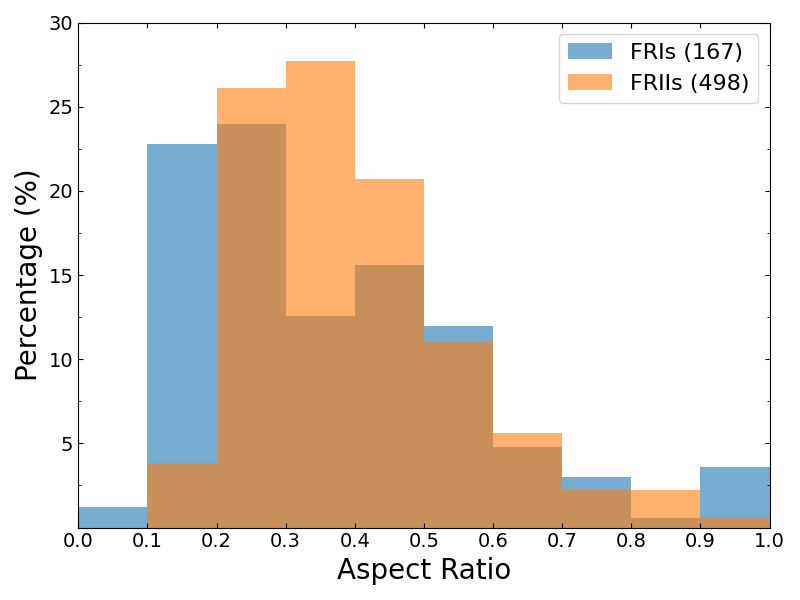
\includegraphics[width=0.9\linewidth]{Figure/Section 4/AxisRatio.png}
    \caption{The vertical axis represents the number of RGs, and the horizontal axis represents the axial ratio of the fitted ellipses. Left Panel: Matching FRIs; Right Panel: Matching FRIIs.}
    \label{fig:Figure7}
\end{figure*}
\begin{figure*}[!htbp]
    \centering
    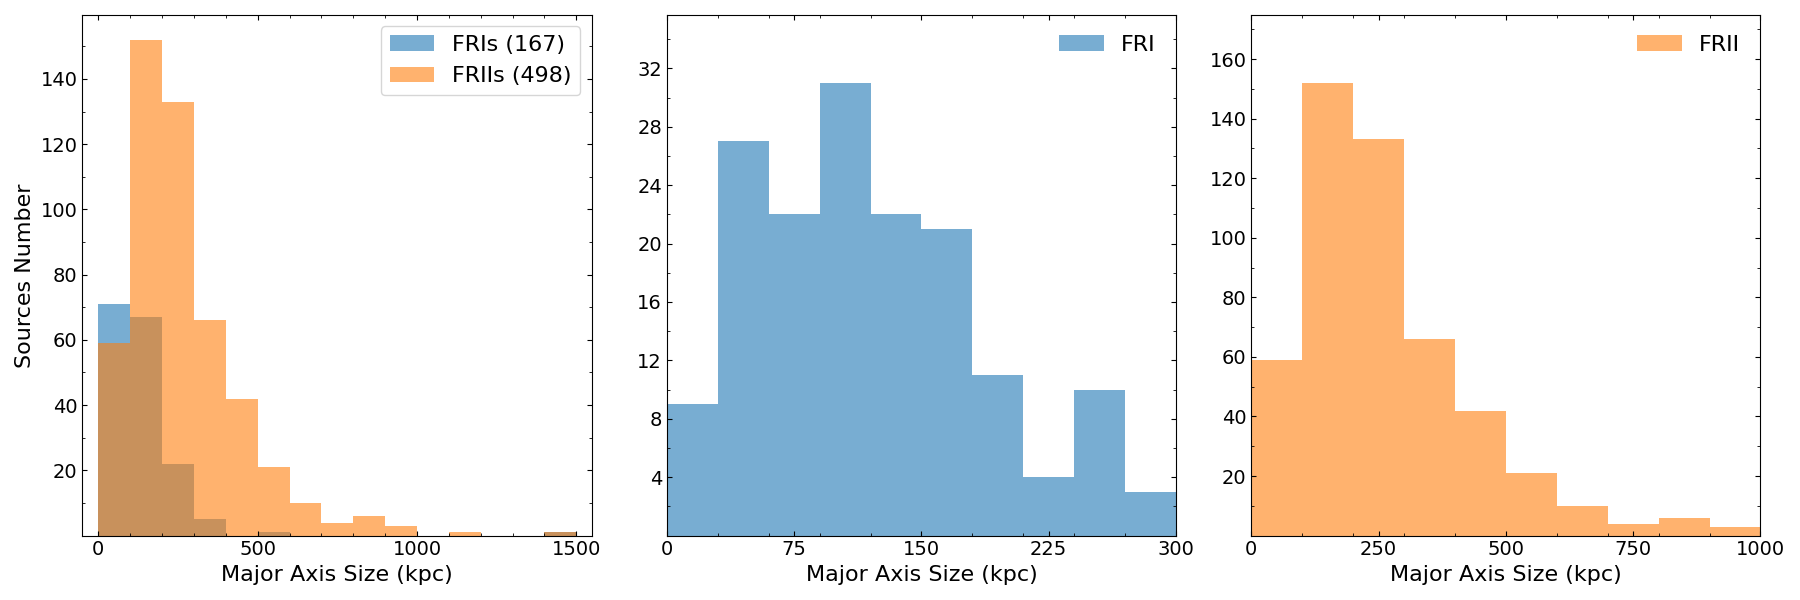
\includegraphics[width=0.9\linewidth]{Figure/Section 4/Max_Scale_Distribution.png}
    \caption{The distribution of intrinsic physical scales of RGs classified by FR type. The blue histogram represents the corrected maximum intrinsic physical scales for FRIs, while the red histogram shows the corrected maximum intrinsic physical scales for FRIIs. The two subplots respectively correspond to enlarged views of the concentration regions of the distributions.}
    \label{fig:Figure8}
\end{figure*}


% Nodes分布特征
\subsection{The Node Structure of FRIs}\label{sec:Section4_2}


\begin{figure*}[!htbp]
    \centering
    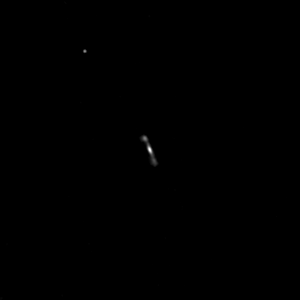
\includegraphics[clip, trim=125 125 125 125, scale=1, width=0.25\linewidth]{Figure/Section 4/Knot_ori.png}
    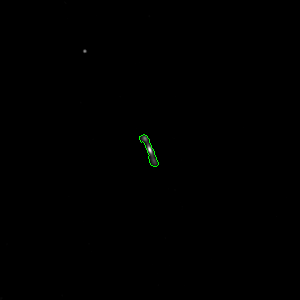
\includegraphics[clip, trim=94 94 94 94, scale=1, width=0.25\linewidth]{Figure/Section 4/Knot_0.5.png}
    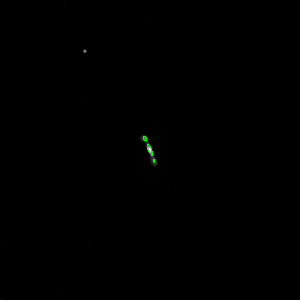
\includegraphics[clip, trim=94 94 94 94, scale=1, width=0.25\linewidth]{Figure/Section 4/Knot_25.png}
    \caption{A FRI type RG located at equatorial coordinates (R.A. 197.092°, Dec. 23.521°). As the threshold increases, four knots are exposed. Left: The original RG (R.A. 178.47°, Dec. 38.197°);  Middle: The contour (Green) of RG;  Right: The contours of clumps when the threshold is 25\%.}
    \label{fig:Figure9}
\end{figure*}

\begin{figure*}[!htbp]
    \centering
    \begin{tabular}{cc}
        \includegraphics[width=0.5\linewidth]{Figure/Section 4/Node_Number.png}& 
        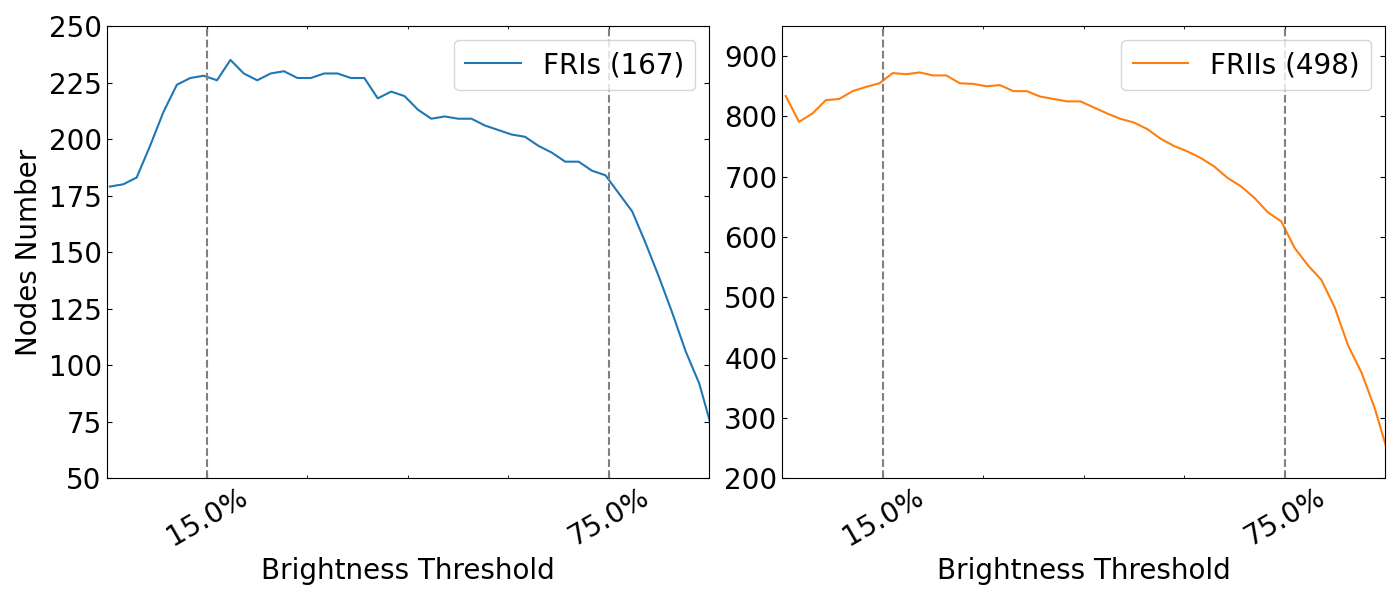
\includegraphics[width=0.45\linewidth]{Figure/Section 4/Node_Evolution.png}\end{tabular}
    \caption{Left Panel: For FRIs, the distribution plot showing the maximum number of nodes appearing as the brightness threshold varies, with the horizontal axis representing the number of nodes and the vertical axis representing the count of RGs possessing that number of nodes; Right Panel: Variation of counts of different types with brightness threshold; The horizontal axis represents the brightness threshold expressed as a percentage of the brightest point in RGs, and the vertical axis denotes the number of RGs or nodes.}\label{fig:Figure10}
\end{figure*}
% \clearpage



\subsection{Classification Parameter $r_s$}\label{sec:Section4_3}



% \begin{figure}
%     \centering
%     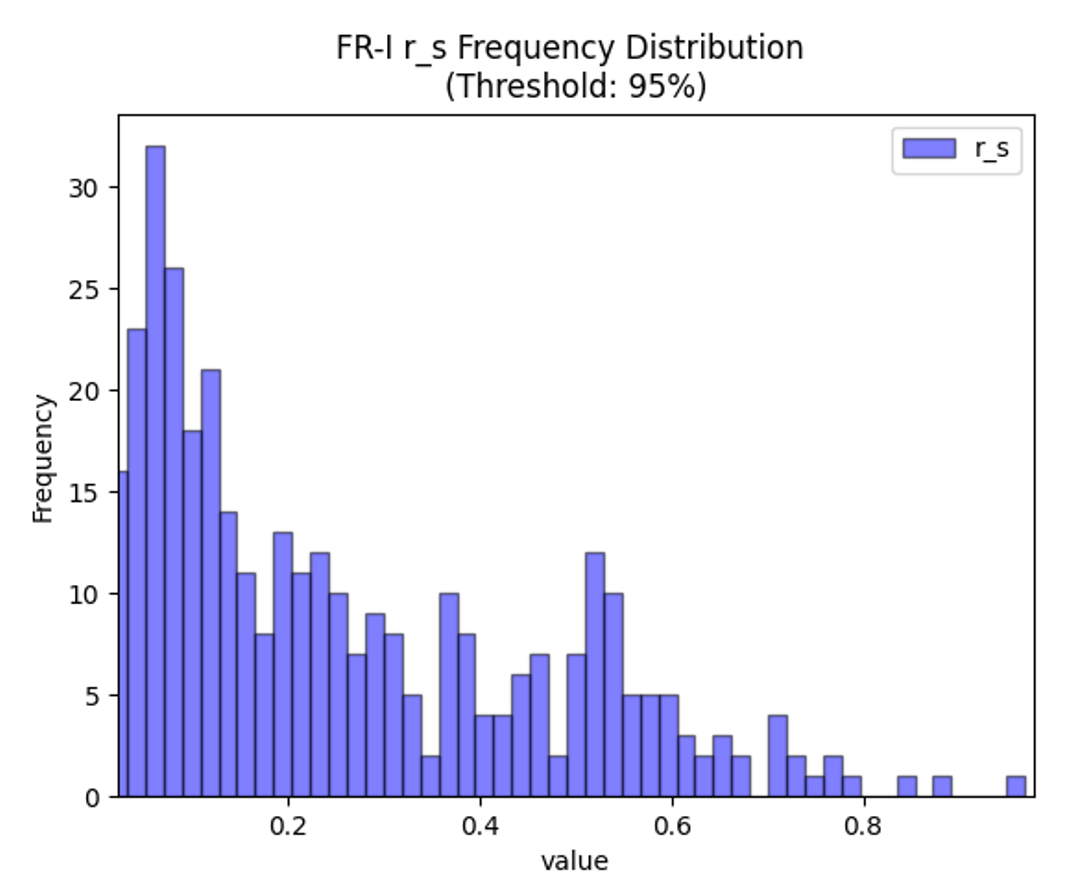
\includegraphics[width=0.9\linewidth]{Figure/Section 4/FR1_rs.png}
%     \caption{Distribution of $r_s$ values for FRIs. The horizontal axis represents the magnitude of $r_s$ values, and the vertical axis denotes the occurrence frequency of RGs corresponding to each $r_s$ value.}
%     \label{fig:Figure11}
% \end{figure}
\begin{figure*}[!htbp]
    \centering
    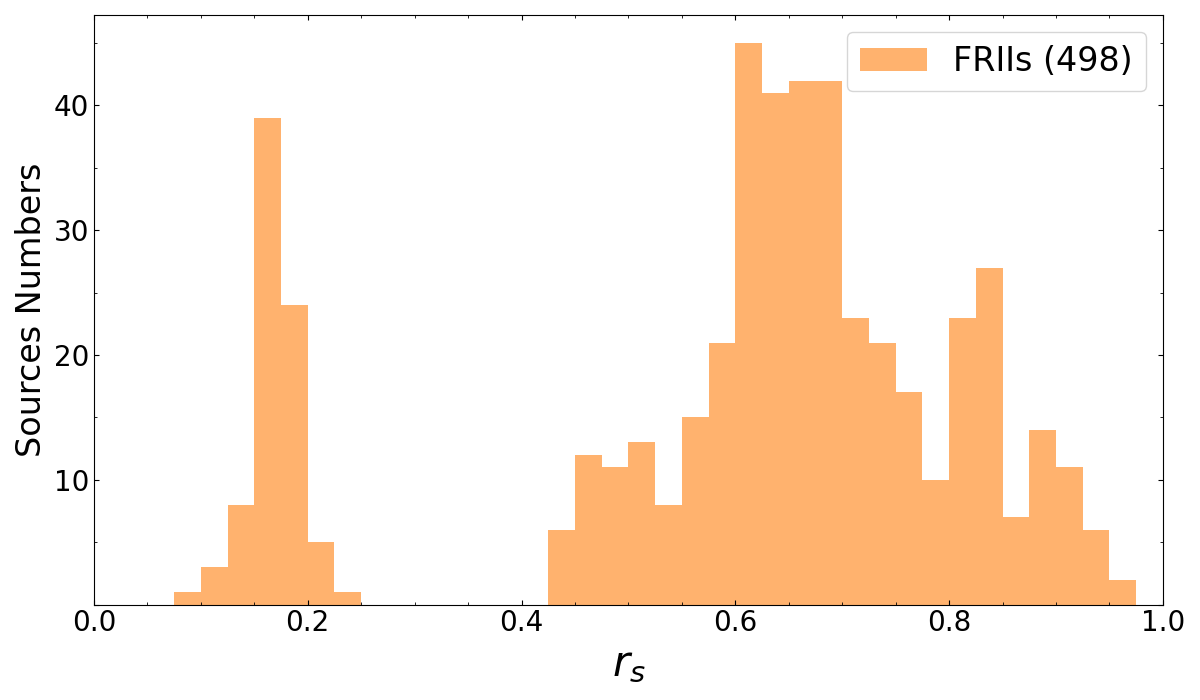
\includegraphics[width=0.45\linewidth]{Figure/Section 4/r_s_distribution0.png}
    \caption{
    Presents the distribution of $r_s$ for brightness thresholds of 95\% (blue) and 50\% (blue, completely obscured by the underlying wine red).
    }
    \label{fig:Figure12}
\end{figure*}
    % 和3D 一起绘制
    % Left Panel: Presents the distribution of $r_s$ for brightness thresholds of 90\% (orange) and 95\% (red, fully obscured by the orange). Right Panel: Presents the distribution of $r_s$ for brightness thresholds of 95\%,90\%,80\%,70\%,60\% and 50\%.



\subsection{The Feature of Central line Brightness Stacking Curve}\label{sec:Section4_4}


\begin{figure*}
    \centering
    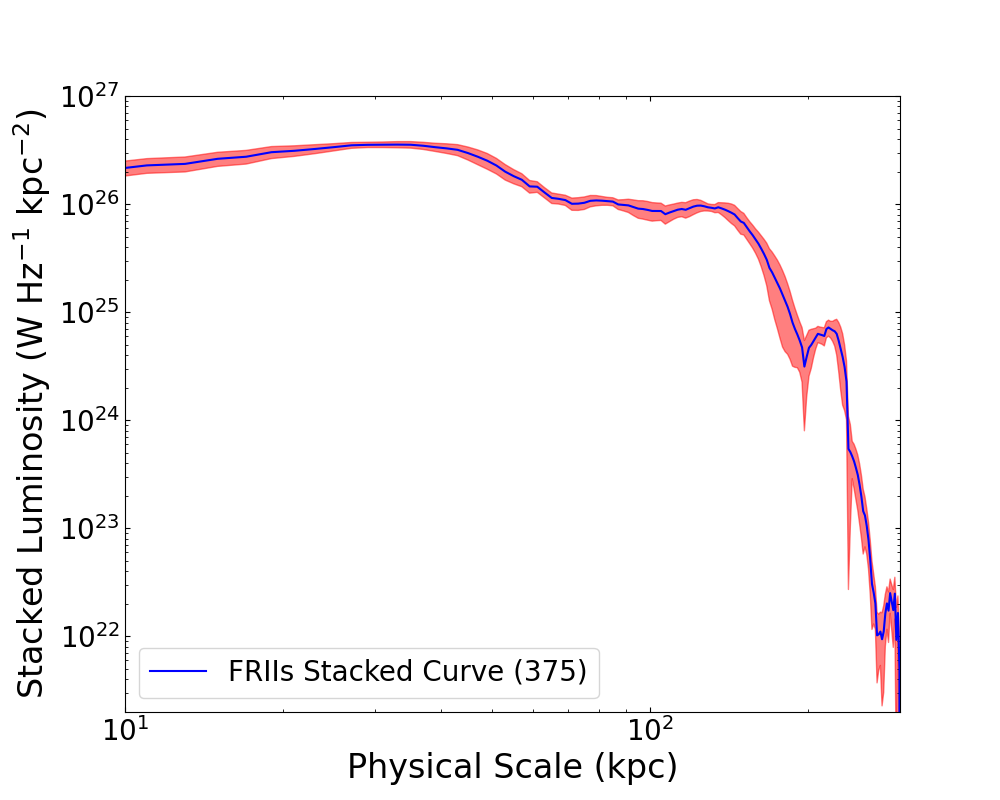
\includegraphics[width=0.45\linewidth]{Figure/Section 4/FR2_StackingCurve1.png}
    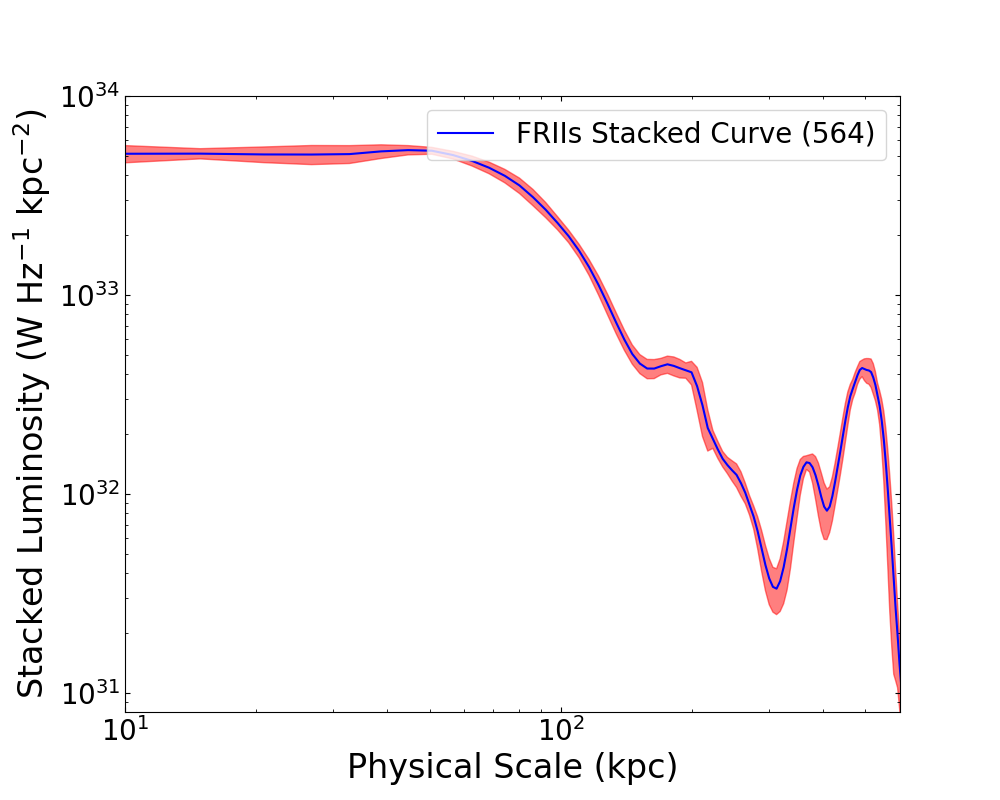
\includegraphics[width=0.45\linewidth]{Figure/Section 4/FR2_StackingCurve2.png}
    \caption{The central line brightness stacking curve of FRIIs. The horizontal axis represents the distance from the extracted physical scales to the location of the optical counterparts of RGs; the vertical axis denotes the logarithmic luminosity.}
    \label{fig:Figure13}
\end{figure*}


% 伸长参数
\subsection{The Distribution of Elongation Parameter}\label{sec:Section4_5}


\begin{figure*}
    \centering
    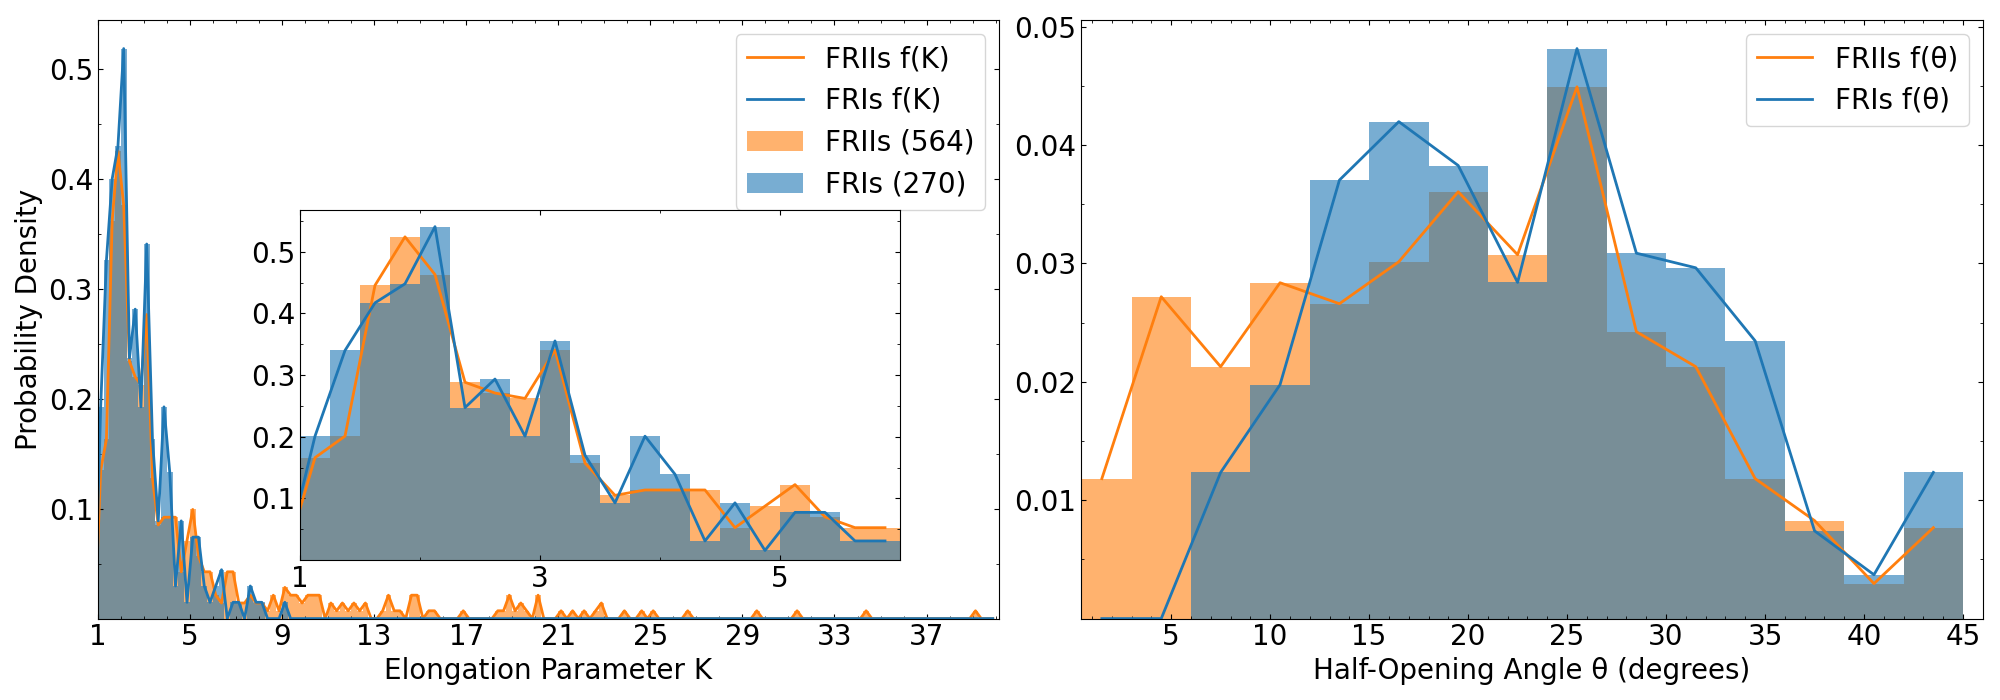
\includegraphics[width=0.9\linewidth]{Figure/Section 4/ProbabilityDensity.png}
    \caption{Left Panel: Probability density distribution of the elongation parameter K; The horizontal axis represents K, and the vertical axis denotes the probability density of K; Histogram bins for K are set at intervals of 0.25, with the corresponding curve $f(K)$ representing the probability density function of K; Red and blue colors correspond to FRIs and FRIIs, respectively. Right Panel: Probability density distribution of the half-opening angles ($\theta$) of RGs estimated using K; The horizontal axis represents the $\theta$, and the vertical axis denotes the probability density of the $\theta$; Histogram bins for the $\theta$ are set at intervals of $3^\circ$ , with the corresponding curve $f(\theta)$ representing the probability density function of the $\theta$.}
    \label{fig:Figure14}
\end{figure*}
% \clearpage


\section{Discussion}\label{sec:Discussion}

\begin{figure}
    \centering
    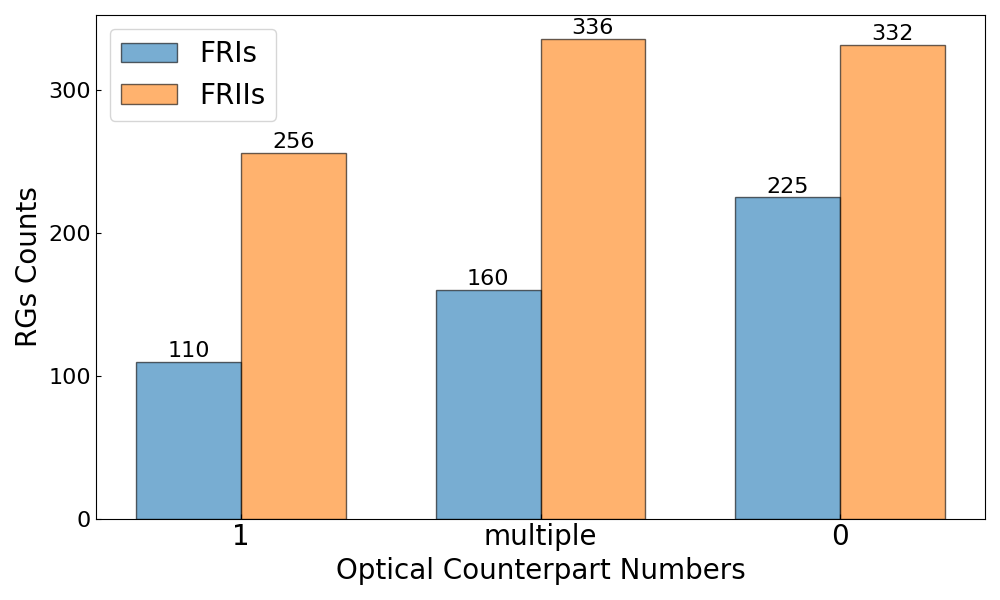
\includegraphics[width=0.9\linewidth]{Figure/Section 5/OpticalCounterpartCountDistributions.png}
    \caption{This figure illustrates the distribution of RGs during the search for their optical counterparts. The two colored labels correspond to FRI/FRII type RGs, respectively. The horizontal axis represents the number of optical counterparts detected for each RG: optical counterparts with a detection count of 1 are relatively more reliable than those with a count of "multiple", and RGs with an optical counterpart count of 0 will be excluded from our subsequent analysis. The vertical axis denotes the number of RGs.}
    \label{fig:Figure15}
\end{figure}
\subsection{The Deviations in Procedure}\label{sec:Section5_1}


\subsection{Similar Mechanism of Morphological Evolution?}\label{sec:Section5_2}




\bibliographystyle{aa.bst}
% \bibliography{BibDir/Introduction.bib,BibDir/Data,BibDir/Method,BibDir/Discussion}
% \bibliography{BibDir/Data,BibDir/Method,BibDir/Discussion}
% \bibliography{BibDir/Introduction.bib}
\begin{appendix}
\section{Alternative thread identification}\label{app:Alt} 




\end{appendix}






\end{document}

